\chapter[A$\beta$42]{Molecular Mechanism of A$\beta$42 fibril inhibition by inositol}

% Some notes
% I found these pretty neat ref articles on sciencedirect
% http://www.sciencedirect.com.myaccess.library.utoronto.ca/science/article/pii/B9780444519672001550
% http://www.sciencedirect.com.myaccess.library.utoronto.ca/science/article/pii/B9780444519672000581
% http://www.sciencedirect.com.myaccess.library.utoronto.ca/science/article/pii/B9780444519672000313
% http://www.sciencedirect.com.myaccess.library.utoronto.ca/science/article/pii/B0080437486011592

	
% \section{Summary}
% Taking away the summary because it's too similar to the previous chapters
% Alzheimer's disease (AD) is a severe neurodegenerative disease with no cure. Currently, one method of targeting the underlying disease is to prevent or reverse the amyloid formation of A$\beta$42, a key pathological hallmark of AD. A small-molecule novel drug candidate, Scyllo-inositol, is a polyol small-molecule that exhibits stereochemistry dependent inhibition of the formation of fibrils in vitro.  Furthermore, recently completed phase II clinical trials demonstrated that scyllo-inositol achieved target drug levels in the cerebral spinal fluid (CSF) of AD patients, a main challenge for AD drug candidates to overcome.
% Despite its promise as a therapeutic for AD, the mechanism of action of scyllo-inositol at the molecular level is currently not understood.  

\section{Introduction}
\abetafortytwo\ is the pathological hallmark of Alzheimer's Disease (AD) and forms the largest proteinaeous component of plaques in the brain of AD patients. \abeta\ peptides are produced from the cleavage of amyloid precursor protein (APP) in isoforms with lengths of 33 to 42 residues. Although A$\beta$42 and A$\beta$40 peptides differ in length only by two residues, \abetafortytwo\ is found to display significantly higher aggregation propensity\cite{Jarrett:1993vm,Fukumoto:1996vi,Finder:2010jw} and cellular toxicity than \abetaforty\ peptides.\cite{ElAgnaf:2000hp,Mucke:2000uqa}
% Furthermore, they are found to form fibrils via distinct pathways.\cite{Bitan:2003ut,Sanchez:2011bj,Bitan:2003p1781}
% Rationale for studying the Abeta42 protofibril system	-- there is all this abeta40 stuff simply because its easier to work with these peptides, but then abeta42 is the actual important peptide that people should be looking at!
Multiple studies have probed the aggregation properties of both \abetaforty\ and \abetafortytwo. Fibril models of the \abetaforty\ peptide derived from solid-state NMR (SSNMR) indicate that protofilaments of \abetaforty\ contain 2 to 3 layers.\cite{Wu:2010p3553,Tycko:2010iz} By contrast, less is known about the fibril structure of \abetafortytwo. A SSNMR-based model of the core of the fibril of \abetafortytwo\ was recently proposed by L\"uhrs et al.\cite{Luhrs:2005p4900} In that model, the cross-$\beta$ core of the fibril consisted of residues 17 to 42, with the N-terminus of the peptide residues 1 to 16 unstructured in the fibril.\cite{Ahmed:2010p5694}
% This doesn't quite belong here.
% A previous MD simulation study based on models of these \abetafortytwo\ protofibrils in pure water suggests that residues 17 to 42 are predominantly involved in the stability of the core structure of the fibril.\cite{Masman:2009p6410}

% Small molecules are promising candidates for the treatment of AD. Many of them have been found to display anti-aggregation activity, including osmolytes.
In recent years, small-molecule inhibitors of \abeta\ amyloid formation have emerged as promising candidates for the treatment of Alzheimer's disease. One such molecule is \textit{scyllo}-Inositol, an inhibitor of A$\beta$42 fibrillation.\cite{McLaurin:2006eb,McLaurin:2000bq,Fenili:2007p3978,Ma:2012jk} Inositol is a class of cyclohexylpolyols, of which eight out of nine stereoisomers are commonly found in nature. \emph{scyllo}-Inositol, in which all hydroxyl groups are equatorial, is the only isomer with two planar hydrophobic faces. By contrast, its diastereisomer, \emph{chiro}-inositol, with two adjacent axial hydroxyl groups, has two nonplanar faces with mixed polarity.
   
\emph{In vitro}, inositol displays stereochemistry-dependent inhibition of A$\beta$42 fibrils: \emph{scyllo}-inositol was shown to inhibit A$\beta$42 fibrillation at concentrations of 1 - 5 mM,\cite{McLaurin:2000bq} whereas \emph{chiro}-inositol is inactive below molar concentrations.\cite{McLaurin:2000bq} Moreover, upon incubation of monomeric A$\beta$42 with \emph{scyllo}-inositol, circular dichroism spectroscopy indicated the formation of $\beta$-sheet structure at an inositol:peptide molar ratio of 25:1.\cite{McLaurin:1998p3149,McLaurin:2000bq}  

Importantly, \emph{scyllo}-inositol was demonstrated to prevent and reverse AD-like symptoms in a transgenic mouse model of AD.\cite{McLaurin:2006eb} Phase I and II of clinical trials for \emph{scyllo}-inositol (ELN0005) in North America has been completed.\cite{Salloway:2011ima,Ma:2012jk} These clinical trials have demonstrated that \textit{scyllo}-inositol possesses positive CNS bioavailability and favorable \emph{in vivo} toxicity profile. Although clinical trials have successfully demonstrated the safety and tolerance profile of \textit{scyllo}-inositol, further chemical modification is likely required to improve its efficacy.  Understanding the structural determinants  of the effect of inositol stereoisomers on A$\beta$42 will aid in the rational design of more efficacious derivatives of inositol.
%Currently, although inositol stereoisomers have been proposed to inhibit amyloid formation by directly interacting with either monomers or non-fibrillar aggregates to ``cap off'' fibril growth,\cite{Janus:2000p198}
However, the molecular basis of the stereospecific effect of \emph{scyllo}- and \emph{chiro}-inositol on A$\beta$42 amyloid inhibition is not understood.
% \cite{Nikolic:2011p185,Rauscher:2006p43,Li:2012p853,Rauscher:2010p5682,Sgourakis:2011hy,Wang:2005do,Cino:2011ff}
% Don't need this -- Molecular dynamics (MD) simulations are well-suited for studies of disordered proteins and can provide atomic-level insight into the mechanism of inhibition of peptide self-aggregation by small molecules. MD simulations were previously employed to examine the binding mechanism of other small-molecule inhibitors such as polyphenols,\cite{Lemkul:2010p23,Wang:2010p204} non-steroidal anti-inflammatory drugs,\cite{Raman:2009p47,Takeda:2010p34} and the well-known amyloid dye thioflavin T\cite{Wu:2008ds,Wu:2011fd} to monomers and/or fibrillar forms of A$\beta$.\cite{Liu:2009p213}

In two previous studies (Chapters 3 and 4), we have successively examined the binding mechanism of \textit{scyllo}-inositol and \textit{chiro}-inositol with peptide and aggregate states of model amyloid-forming peptides\cite{Li:2012bx} and A$\beta$(16-22).\cite{Li:2013fo}  Weak and stereochemistry-independent binding of inositol with the peptidic backbone were found, with binding constants in the range of 0.1 - 1 M, indicating that inositol is unlikely to inhibit amyloid formation by binding the peptidic backbone alone (see Chapter 2).\cite{Li:2012bx} In that initial study, inositol was found to bind to the surface of $\beta$-sheet oligomers with the highest binding affinity, but only more weakly monomeric and disordered morphologies the weakest, suggesting that $\beta$-sheet oligomers are the most likely binding partner of inositol. Upon further investigation with monomeric peptides and aggregates of A$\beta$(16-22), inositol was found to adopt cooperative, high-avidity binding modes with $\beta$-oligomers characterized by binding constants commensurate with \emph{in vitro} inhibitory concentrations.\cite{Li:2013fo}  Taken together, the results from our previous studies indicate that inositol may disrupt amyloid fibrillation by binding to $\beta$-sheet oligomers of A$\beta$.

% Why study with full length ABeta fibrils now - Protofibrils of Abeta(16-22) and full-length protofibrils are different in their physical surface properties.
In this study, we examine successively the binding of inositol stereoisomers, \textit{scyllo}- and \textit{chiro}-inositol, and osmolytes glucose and glycerol with the SSNMR model of the protofibril of full-length \abetafortytwo. Glucose and glycerol are organic osmolytes that can stabilize the folded structures of globular proteins. Osmolytes are thought to stabilize the folded state via the preferential exclusion mechanism.\cite{Bolen:2001im}  In recent years, the osmolytes TMAO,\cite{Seeliger:2013cj} betaine,\cite{Natalello:2009p2237} glucose,\cite{Fung:2005p2008} trehalose\cite{Nayak:2009fr} and glycerol\cite{Sukenik:2011p8778} have been found to modulate amyloid formation and peptide aggregation.\cite{Liu:2005km,Sukenik:2011p8778,Fung:2005p2008,Sukenik:2012dv}
% The molecular basis of cosolute binding to A$\beta$42 fibrils have not been previously examined. 
Here, we compare the binding of inositol stereoisomers, \textit{scyllo}- and \textit{chiro}-inositol with glucose and glycerol, osmolytes which do not inhibit the amyloid formation of A$\beta$42 at sub-osmolar concentration (in the milimolar range or less). Results of this study elucidate the mechanism of action of inositol in the inhibition of A$\beta$ amyloid formation, and shed light on the role of stereochemistry in amyloid inhibition by small molecules in general.
% which will ultimately lead to the development of a pharmcophore for treating AD and related neurodegenerative disorders.
  
\section{Material and Methods} % (fold)
\label{sec:material_and_methods}

The pentameric solid-state NMR model of A$\beta$(17-42) from L\"uhrs \textit{et al.} (PDB code: 2BEG) was taken as the starting structure in our simulations.\cite{Luhrs:2005p4900} In the PDB structure, residues 1 to 16 were truncated in the model because they were found to be disordered.\cite{Luhrs:2005p4900}  The peptides were capped by acetyl groups at the N-terminal end. The acetyl groups were modelled onto the fibril structure using the PyMol software.\cite{Anonymous:2012p58} Titratable amino acids were assigned their charged states at the physiological pH. Ten sodium ions were added to neutralize the remaining charges in the system. To mimic experimental conditions,\cite{Luhrs:2005p4900} 0.15 M (46 ions) of NaCl salt was added. Protein and solvent were represented by the OPLS-AA/L force field\cite{Jorgensen:1996vx} and the TIP3P water model,\cite{Jorgensen:1983p8768} respectively.  The  extended OPLS-AA force field for carbohydrates\cite{Damm:1997tla} was used to model inositol and glucose molecules.

MD simulations were performed in the NpT ensemble using version 4.0.x of the GROMACS simulation package.\cite{Hess:2008p5353} The leapfrog Verlet integration algorithm was used with an integration timestep of 2 femtoseconds. Long-range electrostatic interactions were calculated using Particle Mesh Ewald (PME) summation with a Fourier grid spacing of 0.15 nm and a real-space cutoff of 1.3 nm.\cite{Darden:1993p8963} The short-range nonbonded van der Waals interactions were switched to zero from 1.1 nm to 1.2 nm. The temperature was controlled at 300 K using the Nose-Hoover thermostat.\cite{Nose:1984em} Pressure was controlled by the Parrinello-Rahman barostat at 1 atm with a coupling constant of 4.0 ps.\cite{Parrinello:1981vy} The SHAKE algorithm was used to constrain covalent bonds involving hydrogen atoms.\cite{Ryckaert:1977p9357} Center of mass (COM) rotation and translation were removed at every step.

In all simulations, a cubic box geometry was used with periodic boundary conditions. Prior to data collection, 500 steps of energy minimization using the conjugate gradient algorithm was first performed.  Simulation systems were equilibrated using a two-step procedure.  First, a 200 ps equilibration was conducted in the NVT ensemble to further relax the initial configuration of the system.  Next, equilibration in the NpT ensemble (with isotropic pressure coupling) was conducted for 2 ns to relax the solvent around the protein.

In total, a set of ten 0.250 $\mu$s simulations of the protofibril of \abetafortytwo\ were performed for each of 5 systems,  successively in pure water and in the presence of \textit{scyllo}-inositol, \textit{chiro}-inositol, glycerol and glucose. The ligands were present at a ligand:peptide molar ratio of either 15:5 or 64:5, yielding a total sampling time of 12.5 $\mu$s. 
% See Table XXX for a listing of these simulations.

\subsection{Analysis Protocol}
The GROMACS analysis utilites g\_rmsd and g\_rmsf were used to calculate the root mean square deviation and root mean square fluctuation of the fibril backbone, respectively.  The spatial probability density of bound ligands was computed using the VolMap analysis tool implemented in the Visual Molecular Dynamics (VMD) software package.\cite{Humphrey:1996to}

The number of hydrogen bonds between each pair of peptides in the protofibril was computed using g\_hbond.  The following geometry criteria used to define a hydrogen bond:  (1) the distance between acceptor (A) and donor (D) heavy atoms is less than 0.35 nm, and (2) the angle formed by H-D-A is less than 30$\degreesymb$. Nonpolar contacts between inositol and fibril were defined by a carbon-to-carbon distance cutoff of 0.45 nm. The DSSP algorithm was used to analyze the secondary structure of the protofibril.\cite{Kabsch:1983bp}

\section{Results and Discussion}

We performed simulations of the protofibril of A$\beta$42 successively in the presence of \textit{scyllo}-inositol, \textit{chiro}-inositol, glucose, and glycerol (Figure~\ref{fig:ligands}) at molar ratios of 15:5 and 64:5. In addition, simulations of the protofibril in pure water were also carried out as a control. Because the results were independent of molar ratio, in the sections below, we comparatively examine the binding of the ligands (Figure~\ref{fig:ligands})at the higher molar ratio.

\begin{figure}[htbp]
  \centering
  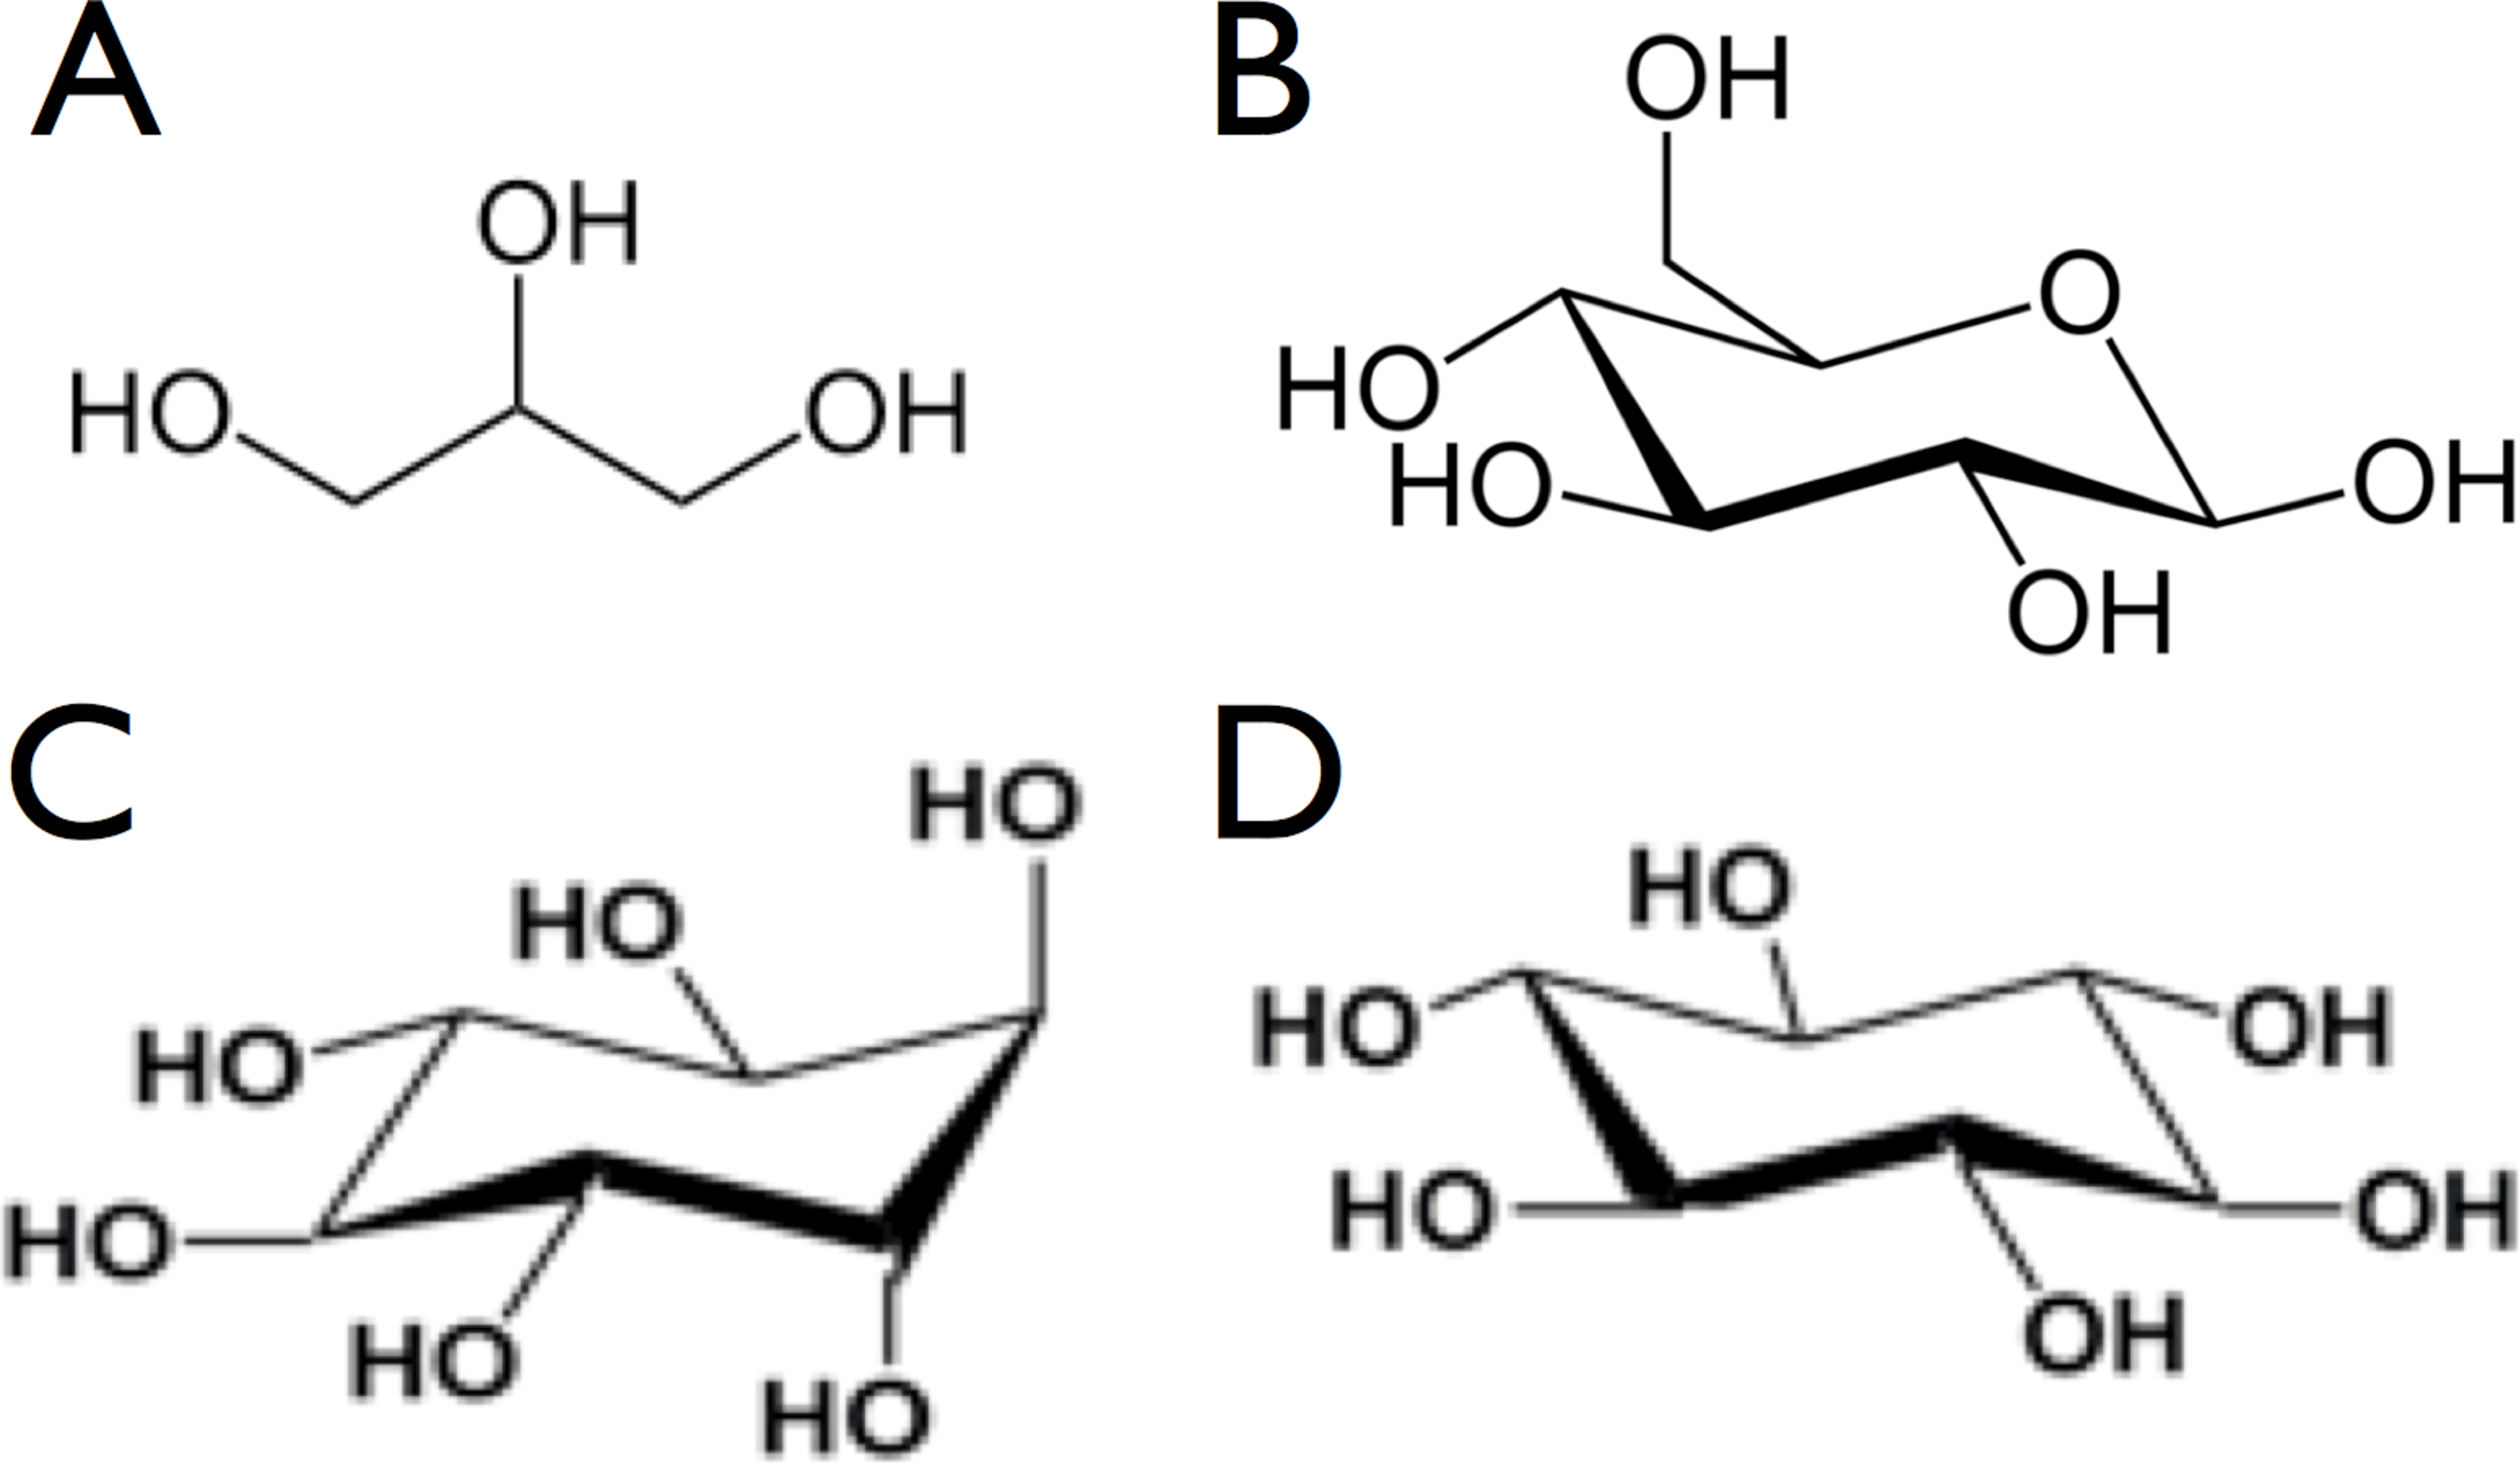
\includegraphics[width=2.5in]{figures/results3/ligands.pdf}
  \caption[Molecular structures of inositol stereoisomers, glucose, and glycerol]{Molecular structures of (A) glycerol, (B) glucose, (C) \textit{chiro}-inositol and (D) \textit{scyllo}-inositol}
  \label{fig:ligands}
\end{figure}

\subsection{Protofibrillar structure}

We first examine the global structural properties of the fibril fragment by examining the time evolution of the RMSD and RMSF (root mean squared fluctuations) of the protofibril. Both in the absence and presence of the ligands (\textit{scyllo}-, \textit{chiro}-inositol, glucose and glycerol) the RMSD of the protofibril over the course of the simulation reached a plateau at ~0.5 nm  (Figure~\ref{fig:protofibril_dynamics}A). The RMSF values depicted in Figure~\ref{fig:protofibril_dynamics}B, shows the average deviation of the position of each residue from its average position. The average RSMF of a residue in the protofibril vary between 0.1 nm and 0.5 nm.  The time evolution of both RMSD and RSMF of the protofibril was independent of the presence and identity of ligands. Although chains at the edges of the fibril were observed to detach partially from the core of the protofibril in some of our trajectories, the $\beta$-sheet core of the peptide aggregate stayed intact throughout the simulation despite the absence of structural restraints. The secondary structure of the protofibril was predominantly $\beta$-sheet. Taken together, these results indicate that the fibril morphology is not significantly affected by the presence of the ligands on the time scale of our simulations. 

\begin{figure}[htbp]
  \centering
  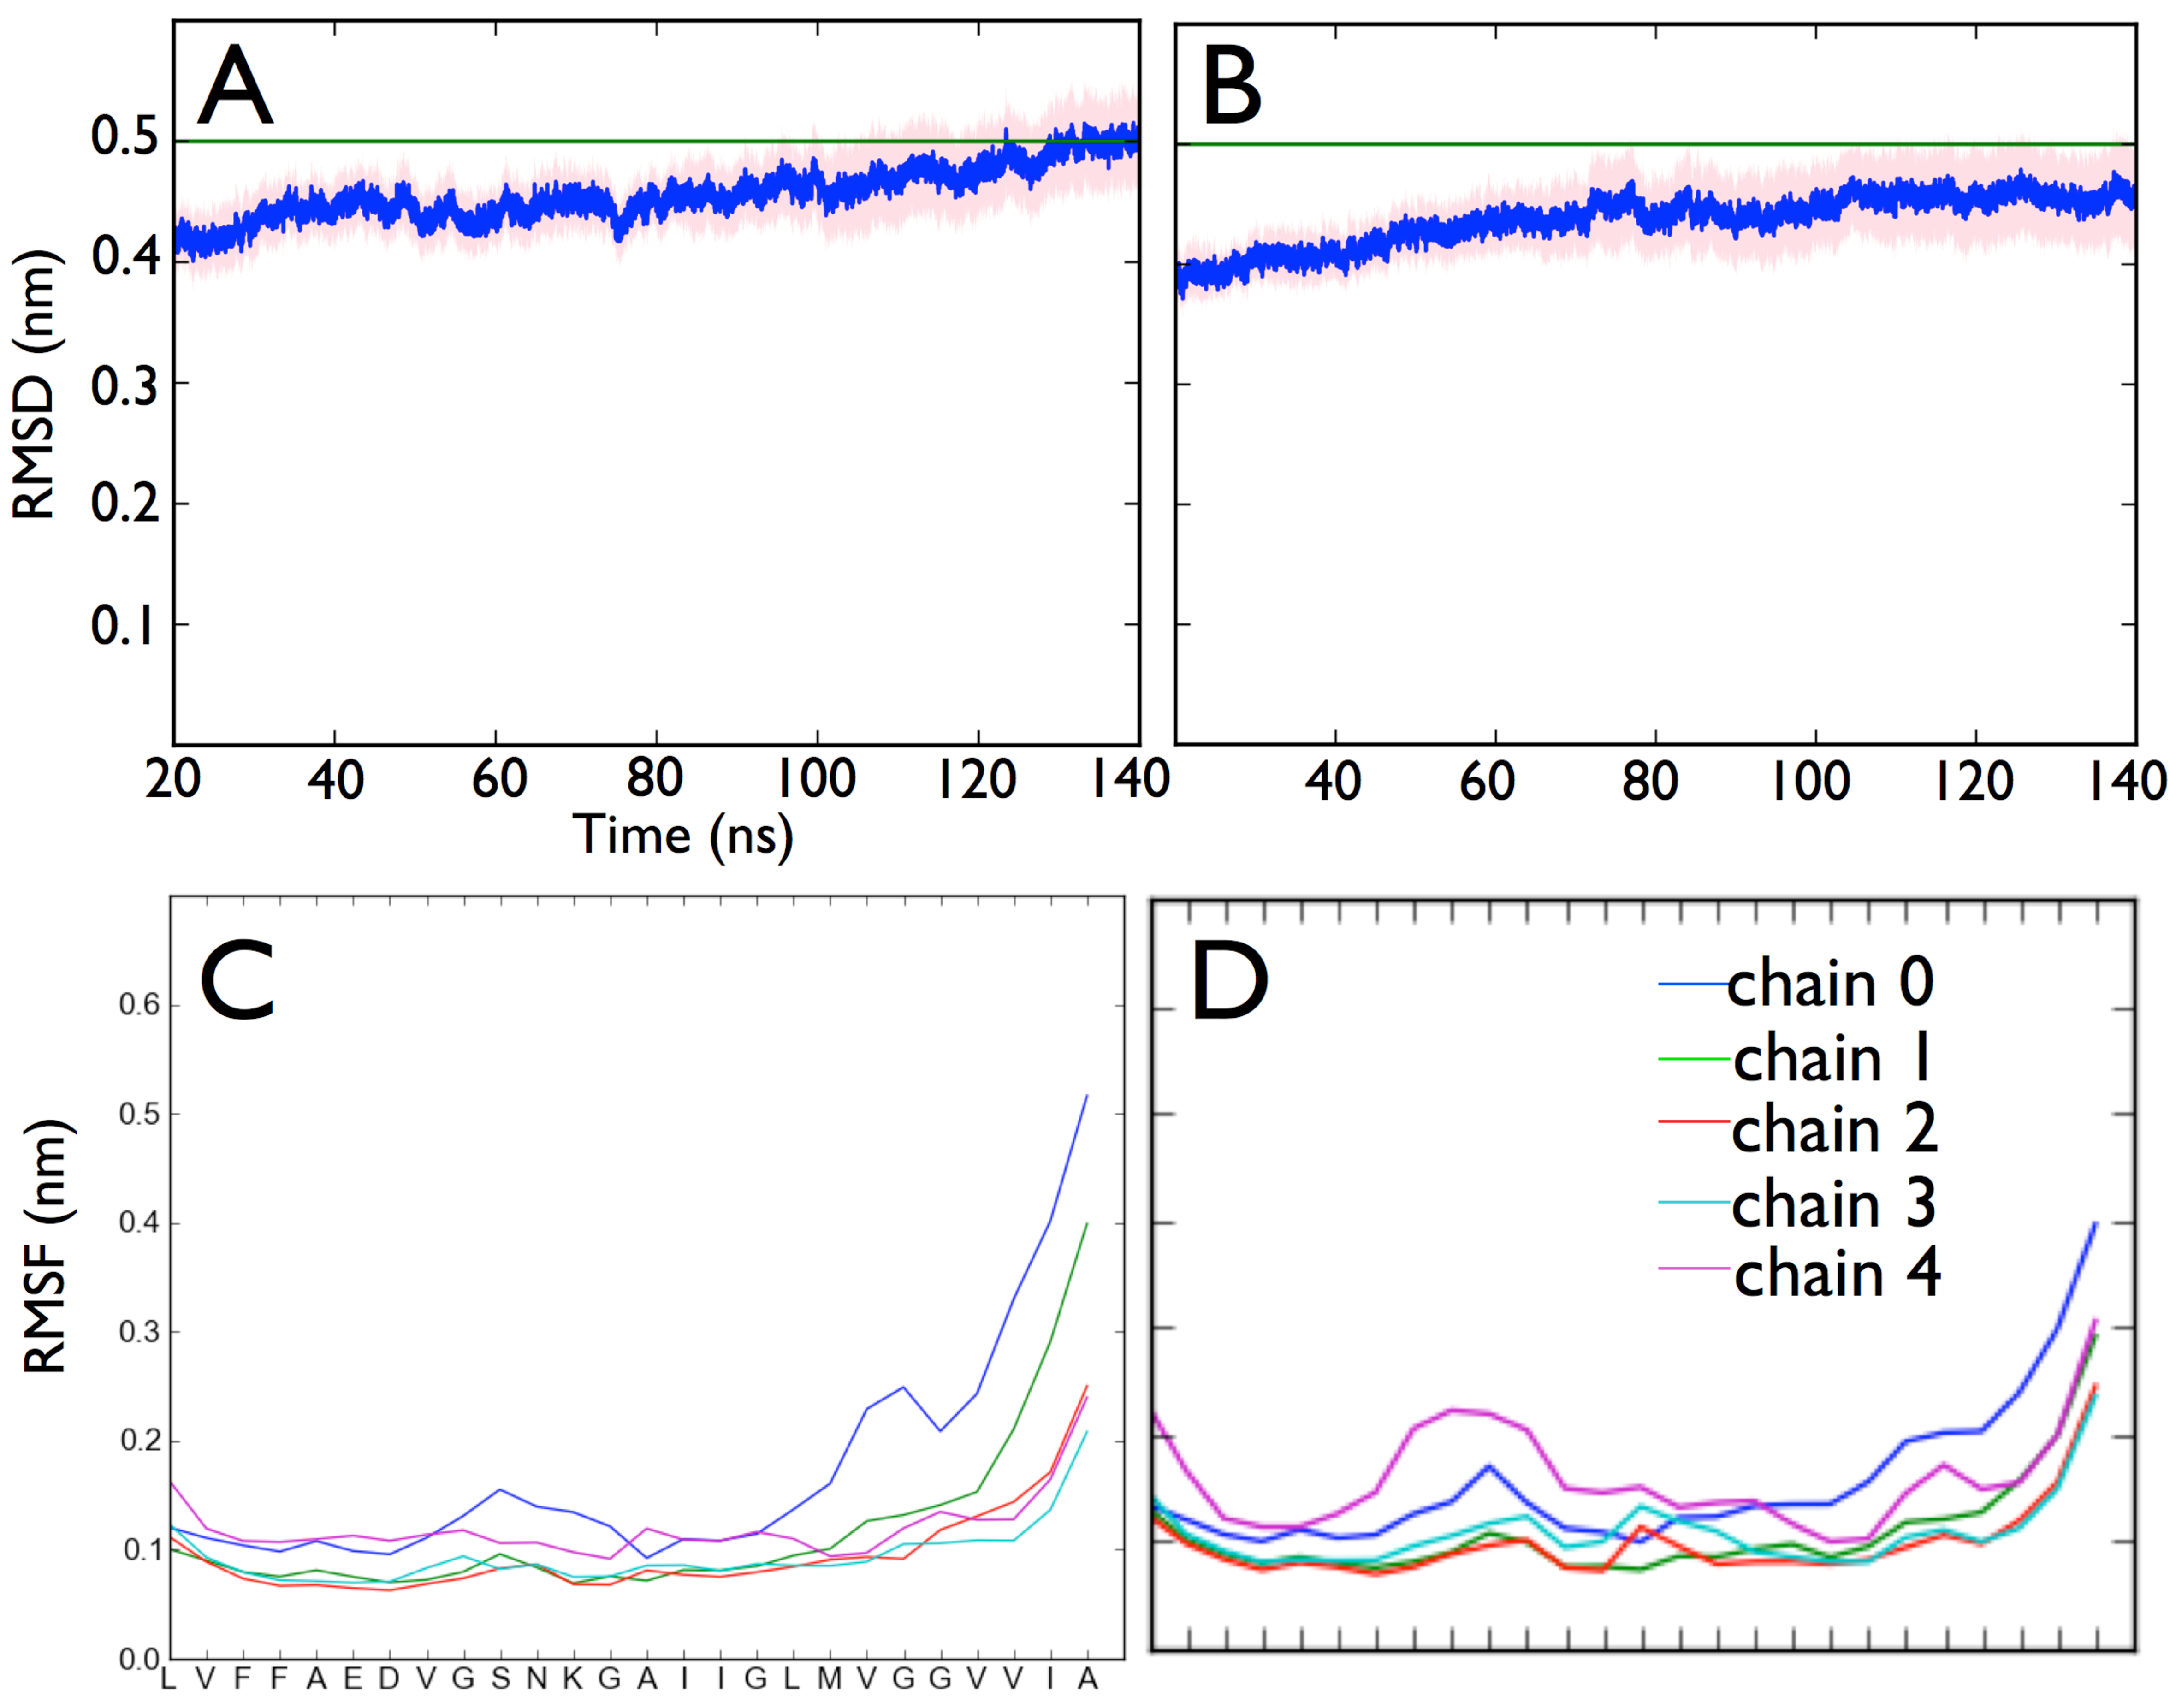
\includegraphics[width=5in]{figures/results3/protofibril_dynamics2.pdf}
  \caption[Protofibrillar morphology]{Fibril structure dynamics in pure water (A and C), and in the presence of \textit{scyllo}-inositol (B and D).}
  \label{fig:protofibril_dynamics}
\end{figure}

\subsection{Ligand binding}
% Qualitative description of the major binding modes
The protofibril presents two chemically different $\beta$-sheet faces. The $\beta$1 face contains residues in the central hydrophobic core of A$\beta$, LVFFA, and possesses a negatively charged region formed by a row of solvent-exposed Glu22 (residue 22 in the full-length peptide). In contrast, the $\beta$2 face presents a predominantly hydrophobic surface containing the residues at the C-terminal end of peptide, IIGLMVGGVVIA (Figure~\ref{fig:protofibril_cartoon}E).  \textit{Scyllo}-inositol, \textit{chiro}-inositol, and glucose molecules all bound to the surface of the protofibril (Figure~\ref{fig:spatial_binding}). Binding involved one or more of four main binding sites on the protofibril: (1) the $\beta$1 face, (2) the $\beta$2 face, (3) the edges, and (4) a channel-like cavity formed between the $\beta$-sheets (Figure~\ref{fig:protofibril_cartoon}).  The binding properties of each of the three solutes in each of these sites and their implication for the mechanism of amyloid inhibition are examined in detail below.

\begin{figure}[htbp]
  \centering
  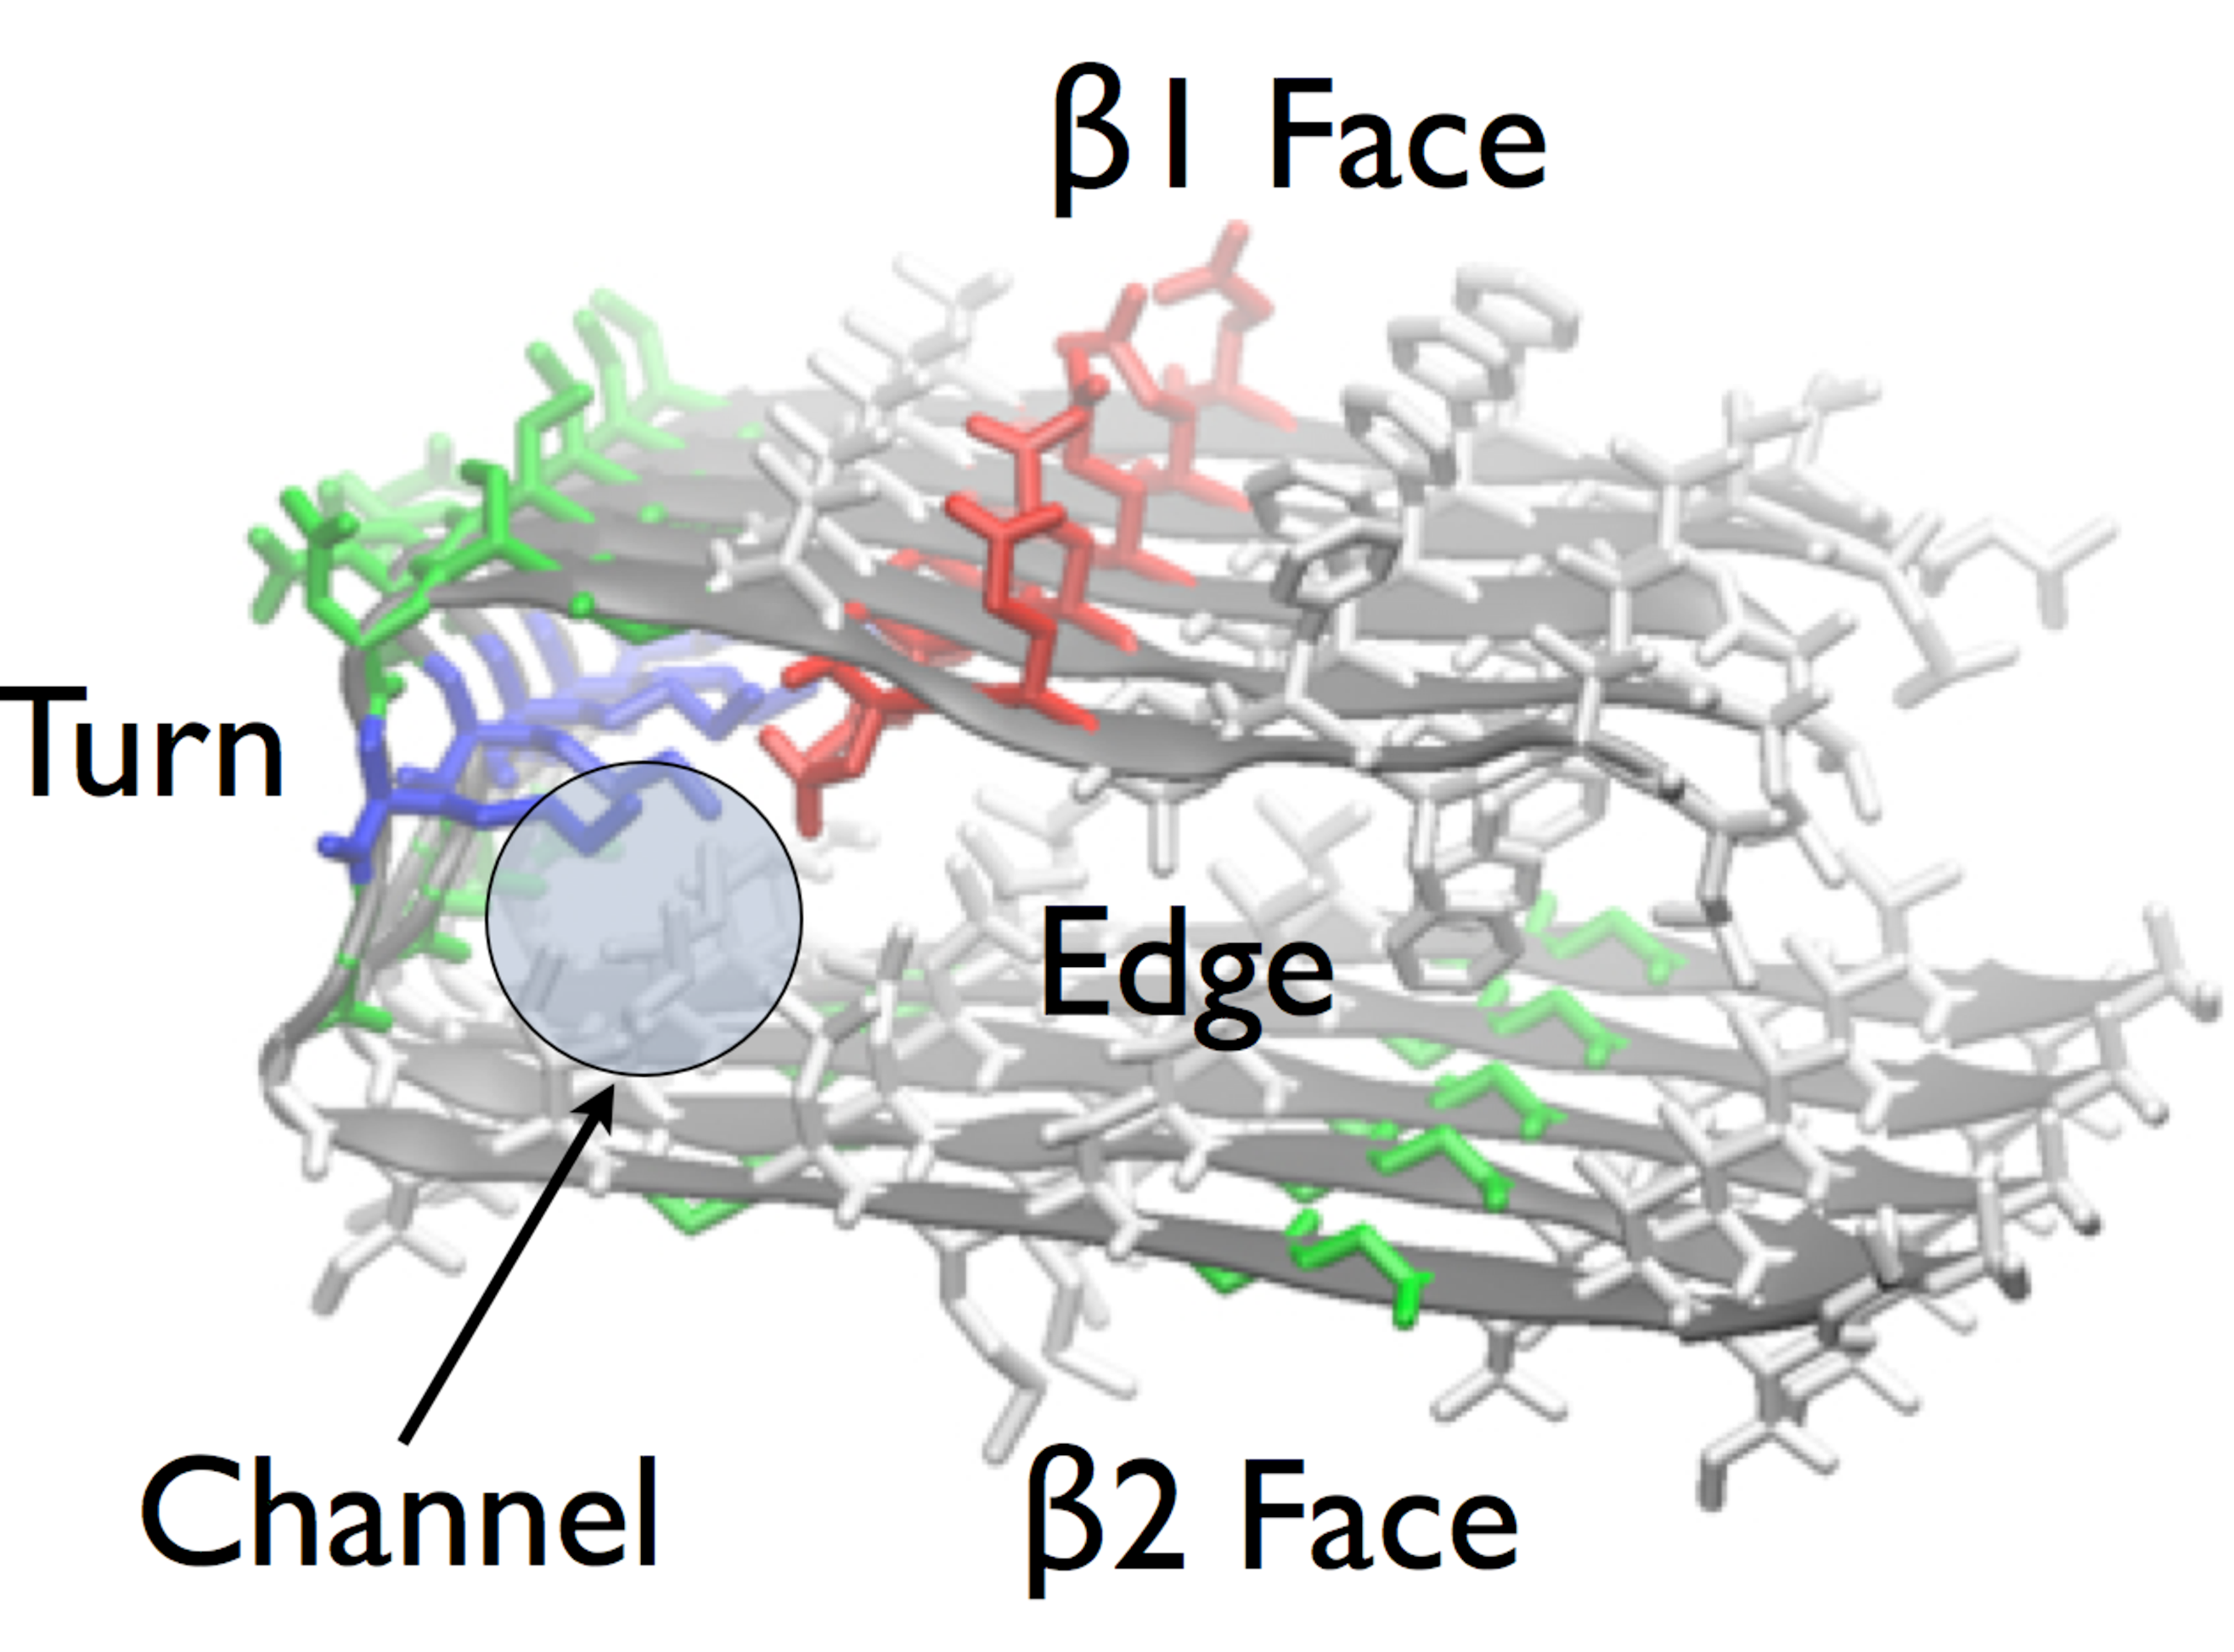
\includegraphics[width=4in]{figures/results3/protofibril_cartoon.pdf}
  \caption[Cartoon representation of the NMR model of the protofibril of A$\beta$42]{The NMR model of the A$\beta$42 protofibril labeled with its major ligand binding sites.}
  \label{fig:protofibril_cartoon}
\end{figure}
 
\textit{Scyllo}-inositol predominantly bound to the $\beta$1 face rather than the $\beta$2 face (Figure~\ref{fig:spatial_binding}A). By contrast, both \textit{chiro}-inositol and glucose show significantly less binding density on the $\beta$1 face, and instead were bound predominantly to the $\beta$2 face.  Contact maps of ligand-protofibril binding indicate that binding on the $\beta$1 face is localized to residues Phe20 and Glu22 (Figure~\ref{fig:binding_map}).  As depicted in Figure~\ref{fig:detailed_binding_modes}, all three molecules adopt binding modes to the $\beta$1 face via a combination of hydrogen bonding to Glu22 and nonpolar contacts with Phe20. However, \textit{scyllo}-inositol is the only ligand which can adopt a face-to-face binding mode with the side chain of Phe20 while simultaneously hydrogen bonding with Glu22. This binding mode has been characterized in our previous study in Chapter 4.\cite{Li:2013fo}

Contrary to both inositol and glucose, glycerol did not display significant binding density on either face (Figure~\ref{fig:spatial_binding}C). Because glycerol did not bind to the solvent-exposed surface of the protofibril, unless otherwise specified, the term ligands will be used to collectively refer to \textit{scyllo}-, \textit{chiro}-inositol and glucose for clarity in the sections below.

\begin{figure}[htbp]
  \centering
  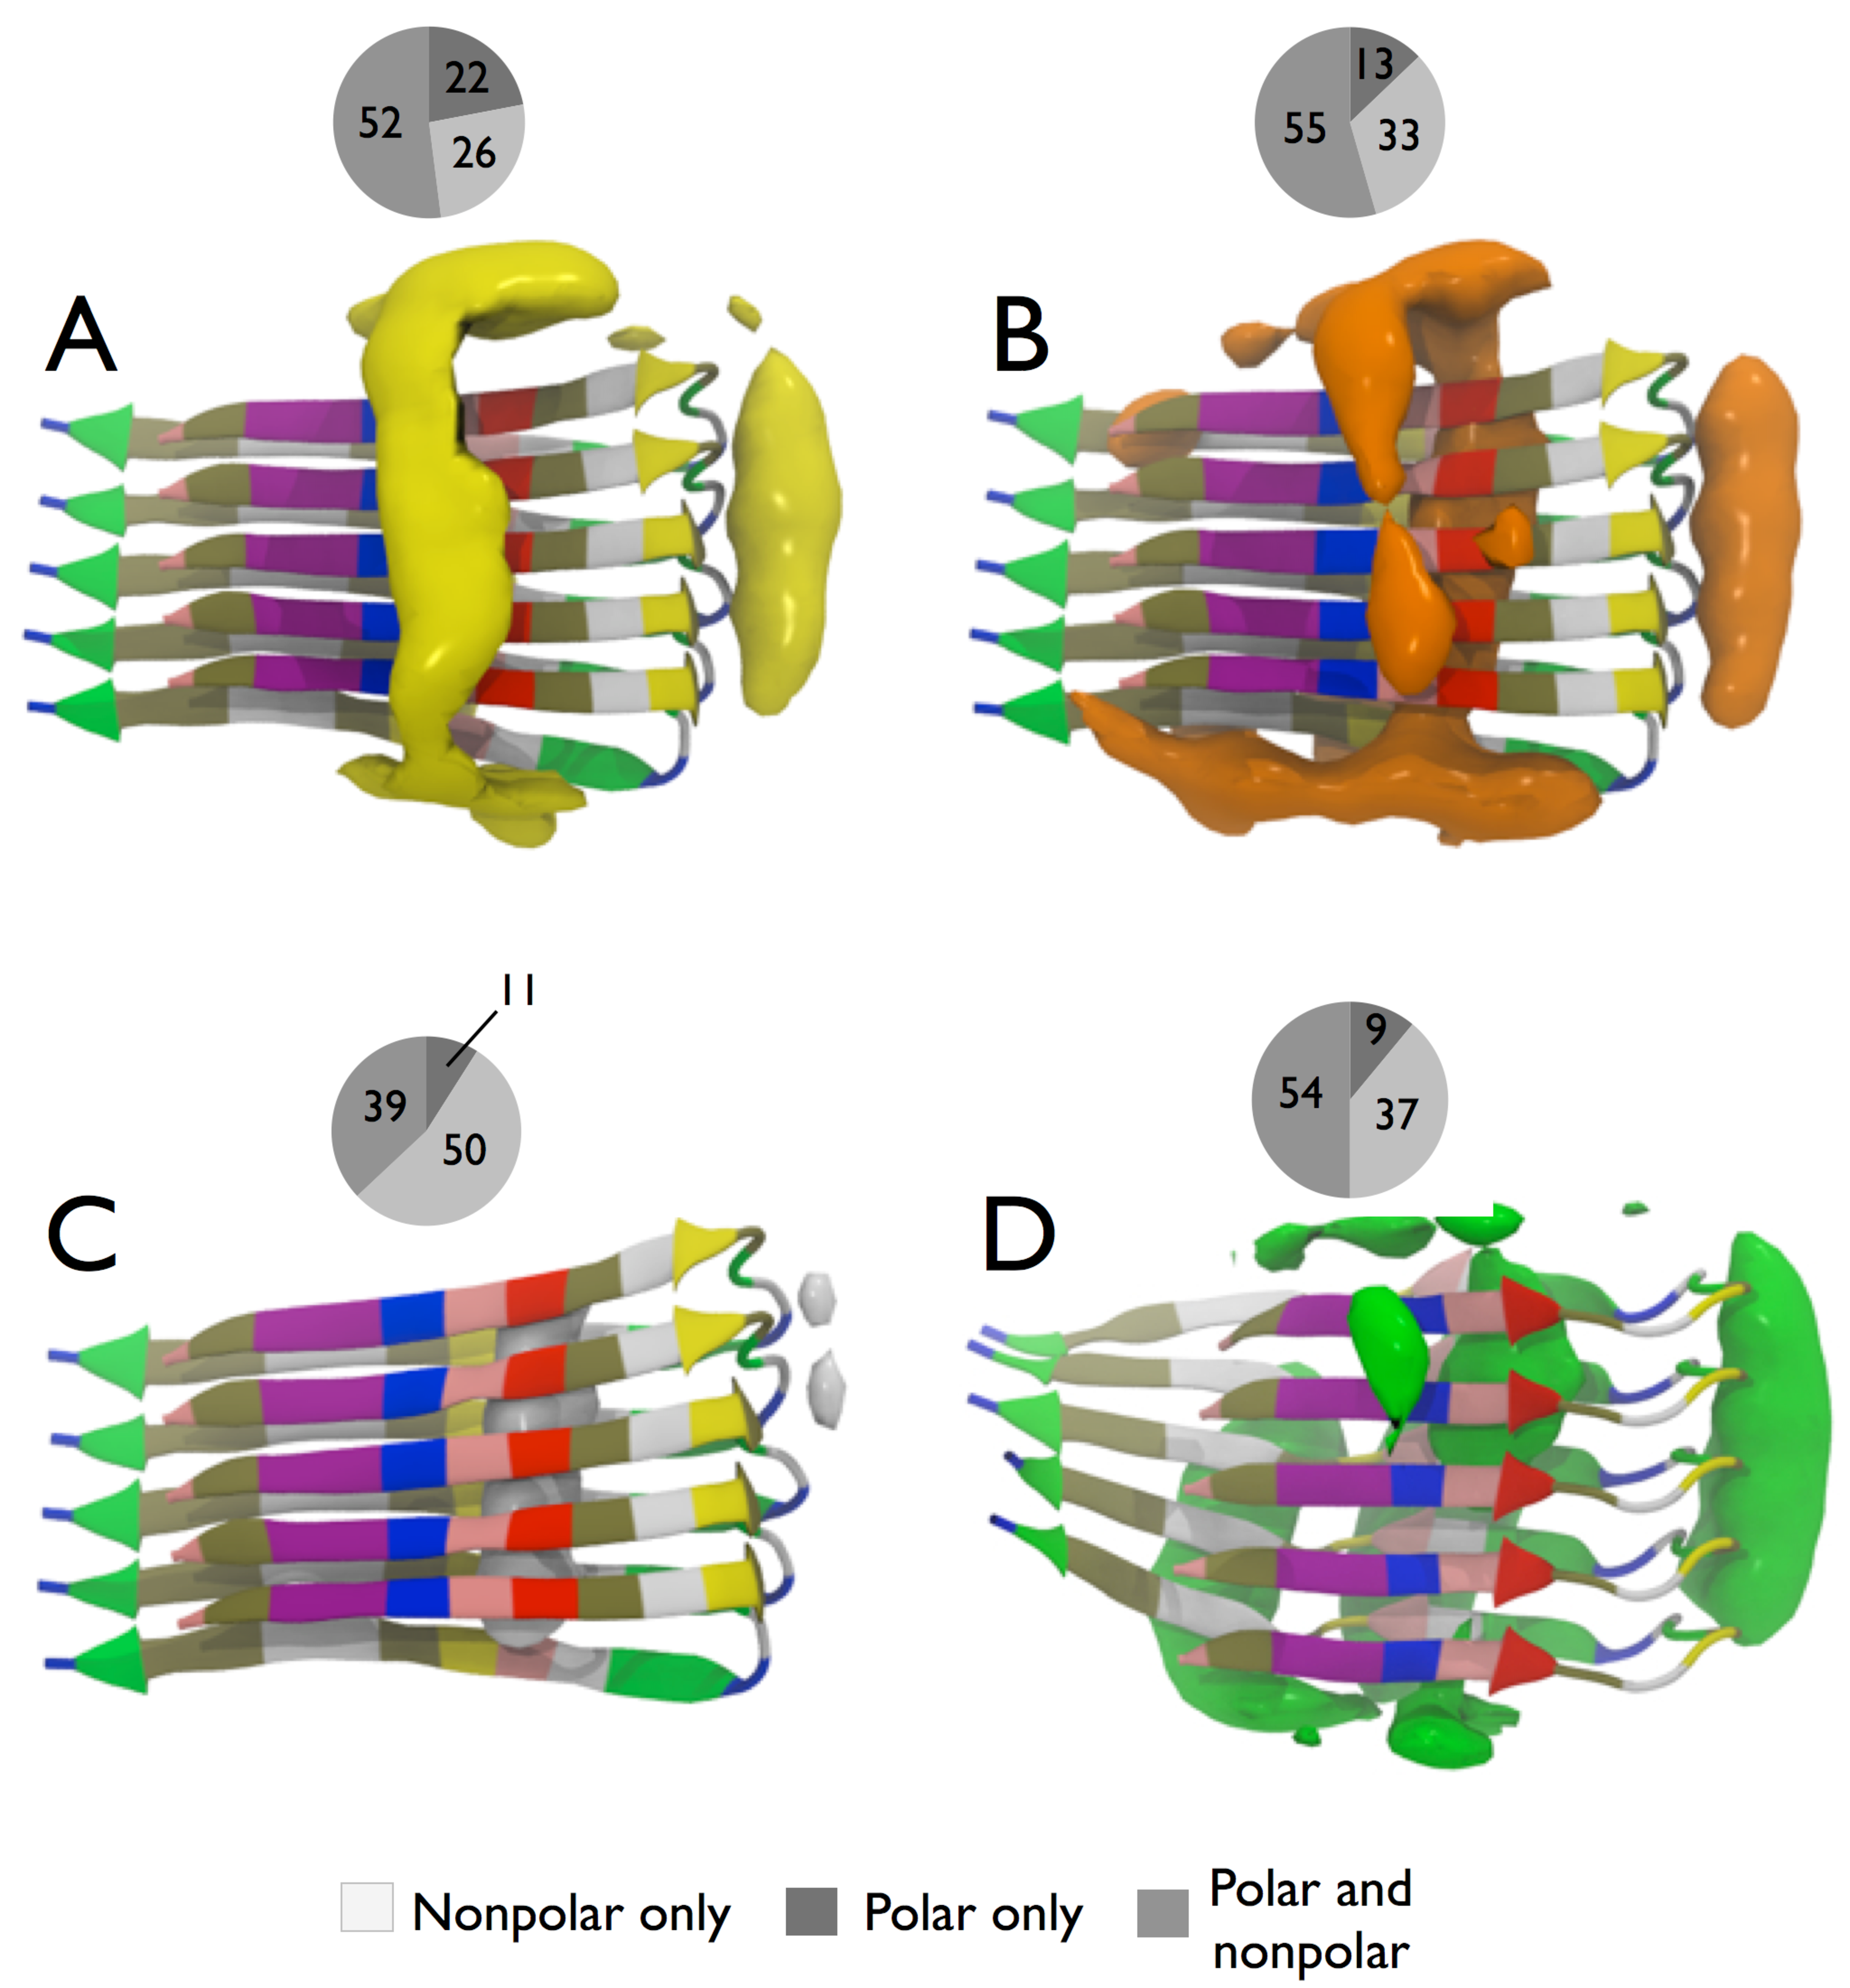
\includegraphics[width=6in]{figures/results3/binding_sdf_pie_chart.pdf}
  \caption[Spatial probability distribution of bound solutes]{Comparison of the spatial binding probability densities and binding modes for (A) \textit{scyllo}-inositol, (B) \textit{chiro}-inositol, (C) glycerol and (D) glucose.}
  \label{fig:spatial_binding}
\end{figure}

Another binding site with significant binding density is found in the grooves located at the edges which runs parallel to the $\beta$-strands in the protofibril. Again, \textit{scyllo}-inositol displayed a narrower and more localized density than those of \textit{chiro}-inositol (Figure~\ref{fig:spatial_binding}, \ref{fig:binding_map}), which bound non-specifically to residues along the entire edge.  By contrast to the inositol stereoisomers, glucose did not bind to the edges significantly. Based on these results, we speculate that binding at the edges may slow down fibril elongation, but is unlikely to lead to arrest of the growth of a protofibril into amyloid fibrils.
%\textbf{The ligand-protofibril contact maps shown in Figure~\ref{fig:} indicate that ...[ elaborate - which residues? Look at the contact map ].}

\begin{figure}[htbp]
  \centering
  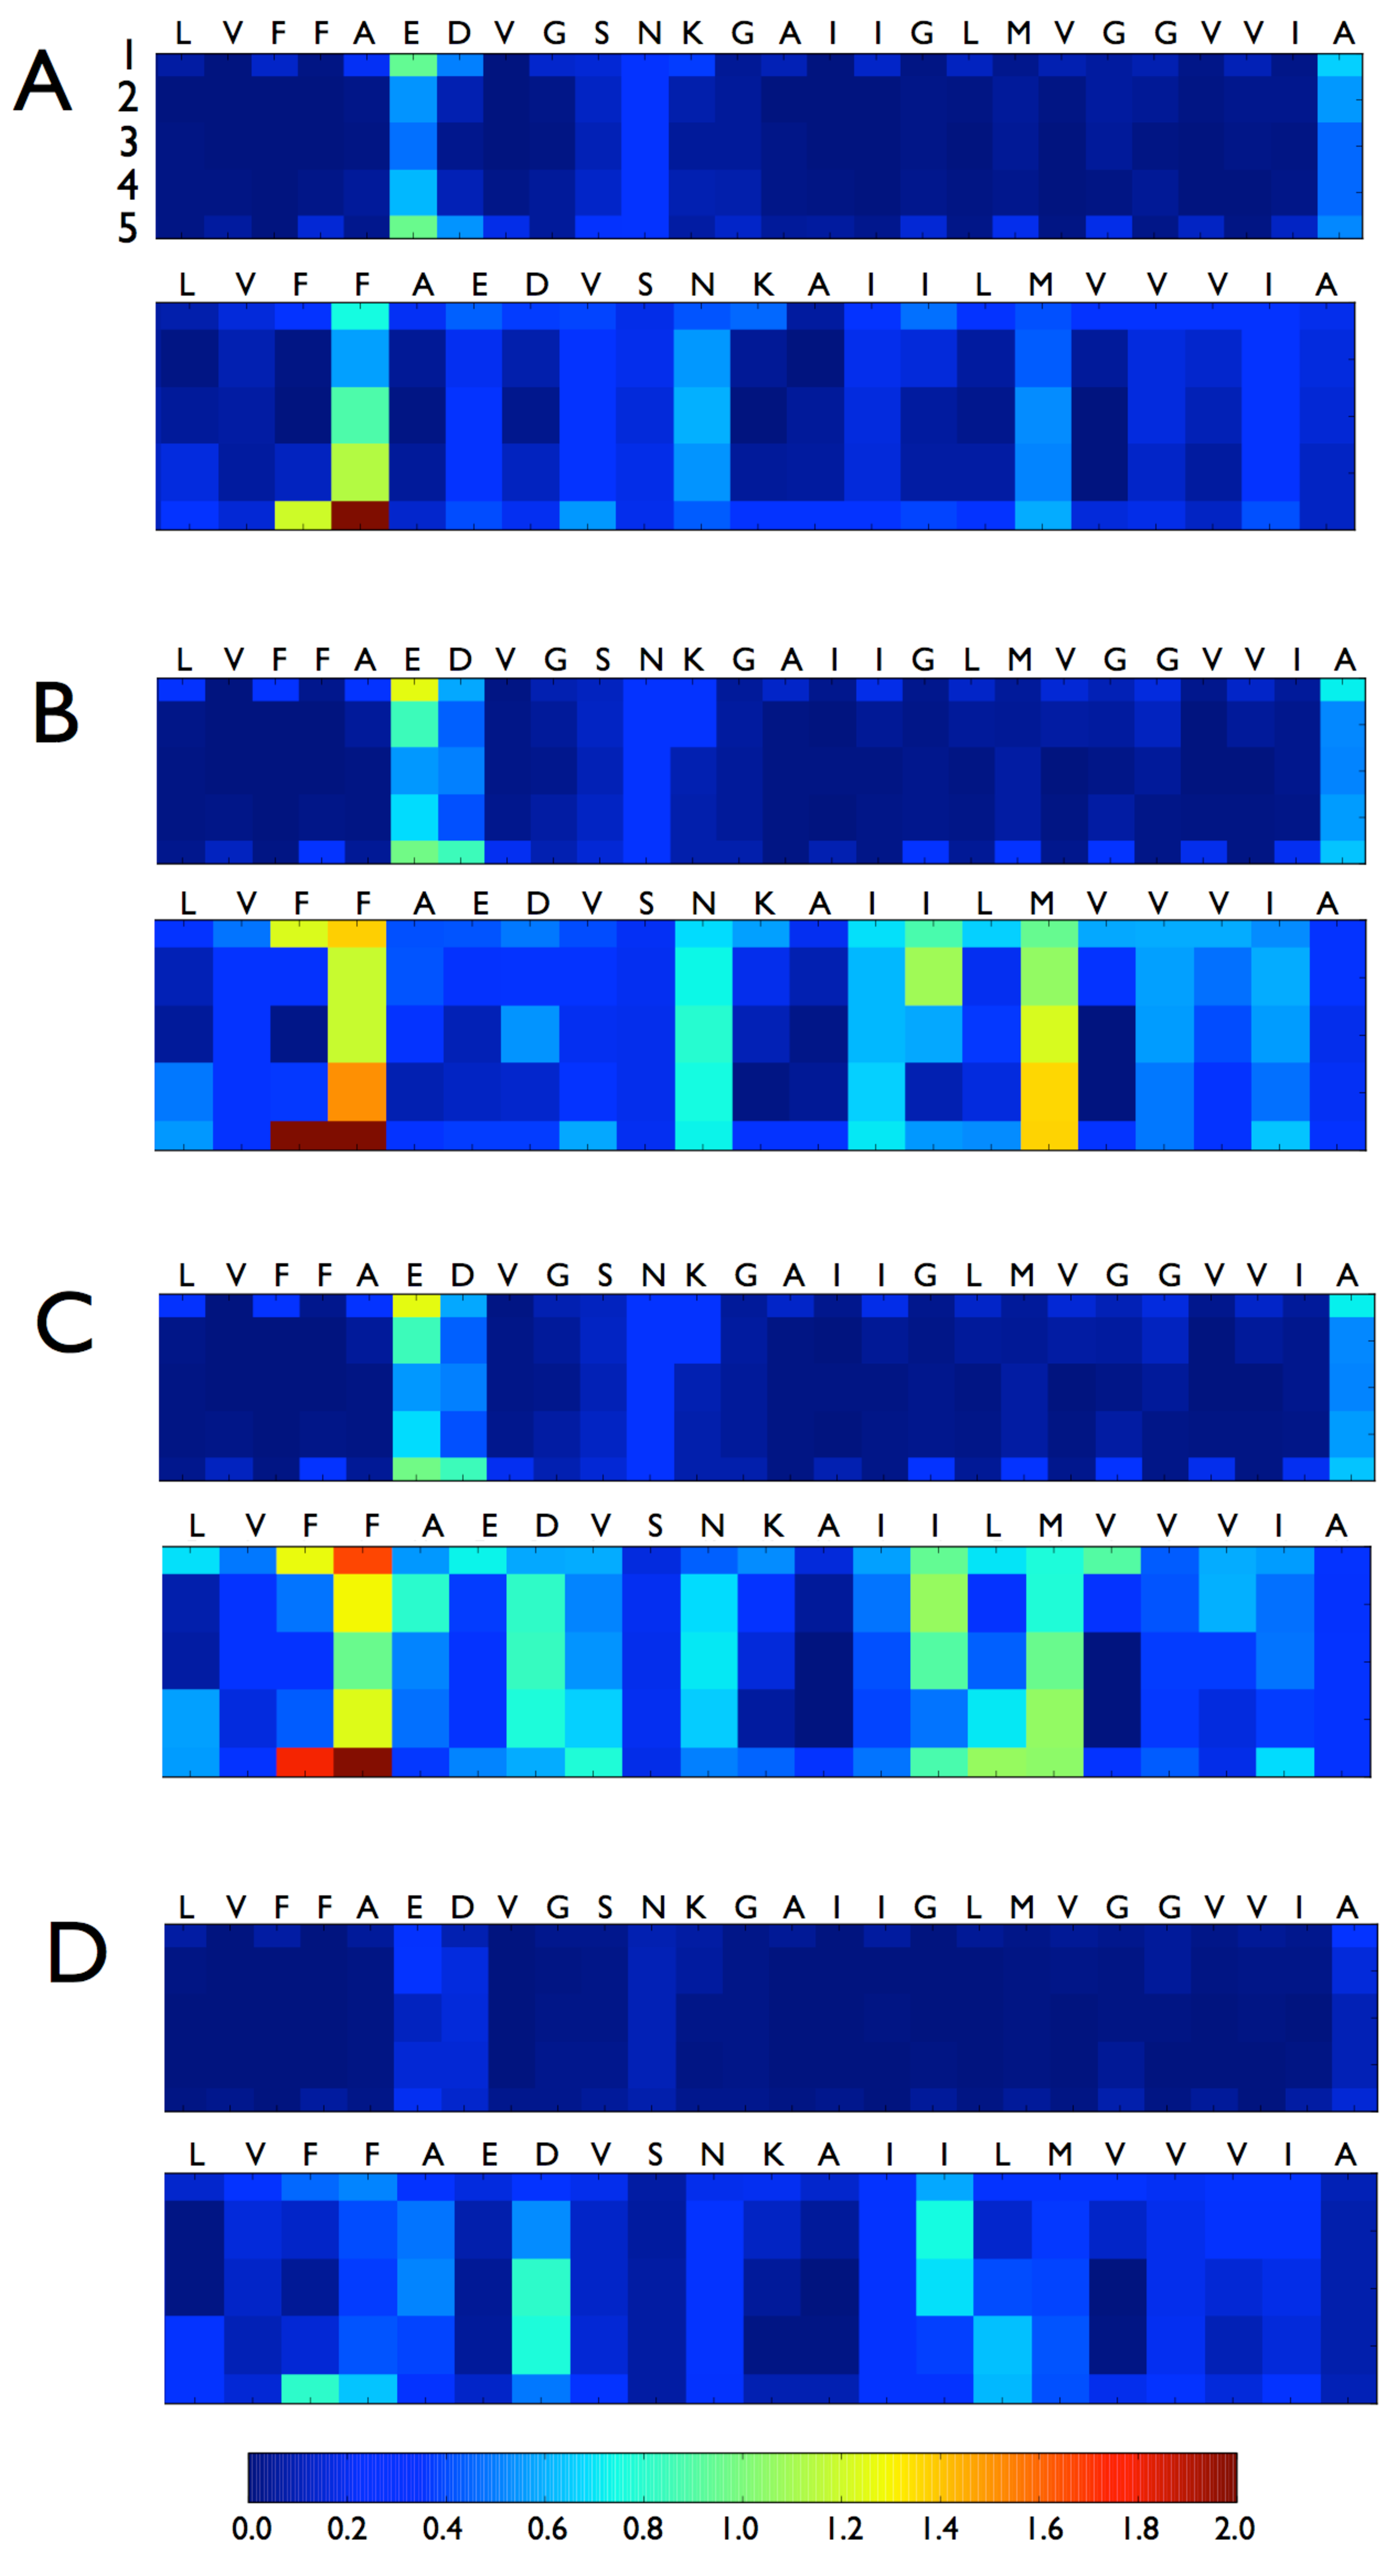
\includegraphics[width=4in]{figures/results3/binding_maps_horizontal.pdf}
  \caption[Binding contact map]{Contact maps for ligand-protofibril binding involving hydrogen bonding (top) and nonpolar contact maps (bottom) for (A) \textit{scyllo}-inositol, (B) glucose, (C) \textit{chiro}-inositol, and (D) glycerol. Each row and column of the matrix represents the average number of contacts for a peptide and a residue in the protofibril, respectively.}
  \label{fig:binding_map}
\end{figure}

% Binding in the channel
Furthermore, the protofibril exhibits a intersheet channel-like cavity formed by residues 8 - 19 of the peptide (Asp8, Val9, Gly10, Ser11, Asn12, Lys13, Gly14, Ala15, Ile16, Ile17, Gly18, and Leu19), which together adopt a turn conformation (Figure~\ref{fig:protofibril_cartoon}).  Of these residues, only the side chains of Asp23, Lys28, Ile32, and Leu34 line the inside of the cavity.  \textit{Chiro}-inositol, glucose, and glycerol, unlike \textit{scyllo}-inositol displayed significant binding densities here (Figure~\ref{fig:spatial_binding}).
% Does not happen with glycerol - completely nonspecific. Scyllo only specific to FAE region.
Both \textit{chiro}-inositol and glucose bound on the inside of the channel by forming linear-hydrogen-bonded chains (Figure~\ref{fig:detailed_binding_modes}) that simultaneously formed hydrogen bonds and nonpolar contacts with side chains of residues inside the channel.  Although \textit{chiro}-inositol and glucose  penetrated this cavity, \textit{scyllo}-inositol instead was mostly trapped near its entrances (Figures~\ref{fig:spatial_binding}, \ref{fig:detailed_binding_modes}).
% Although scyllo-inositol can intercalate between the sheets near the opening of this tunnel, a significant binding density for scyllo-inositol was not found on the inside (Figure~\ref{snapshot of scyllo binding at this region}). 
In support of our results, several previous simulation studies utilizing the same model of the A$\beta$42 protofibril have observed similar binding modes for amyloid dye molecules (ThT and PiB),\cite{Wu:2011fd} and a polyphenol morin.\cite{Lemkul:2010p6251} Differential binding in this cavity exhibited by the inositol stereoisomers and glucose indicates how the stereochemistry of small molecules can modulate their binding to amyloid morphologies.
% TODO AND what???
%In corroboration with our results, a MD study by Shea et al. indicated that dye molecules, PiB and ThT,  can penetrate into the same channel for the same protofibrillar model.\cite{Wu:2011fd} (This sentence is better for discussion). -- SO WHAT?
% Although small molecules can bind inside the protofibril, these binding modes is unlikely to disrupt the integrity of the protofibril.
We hypothesize that these binding modes are unlikely to lead to amyloid inhibition, as these binding sites are not located at an area where fibril growth may occur. Furthermore, we speculate that binding in this region may be an unproductive binding mode, which may serve to decrease the inhibitory activity of small molecules. Accordingly, the non-inhibitors, glucose and \textit{chiro}-inositol, were more prone to participating in these binding modes.  

\begin{figure}[htbp]
 \centering
 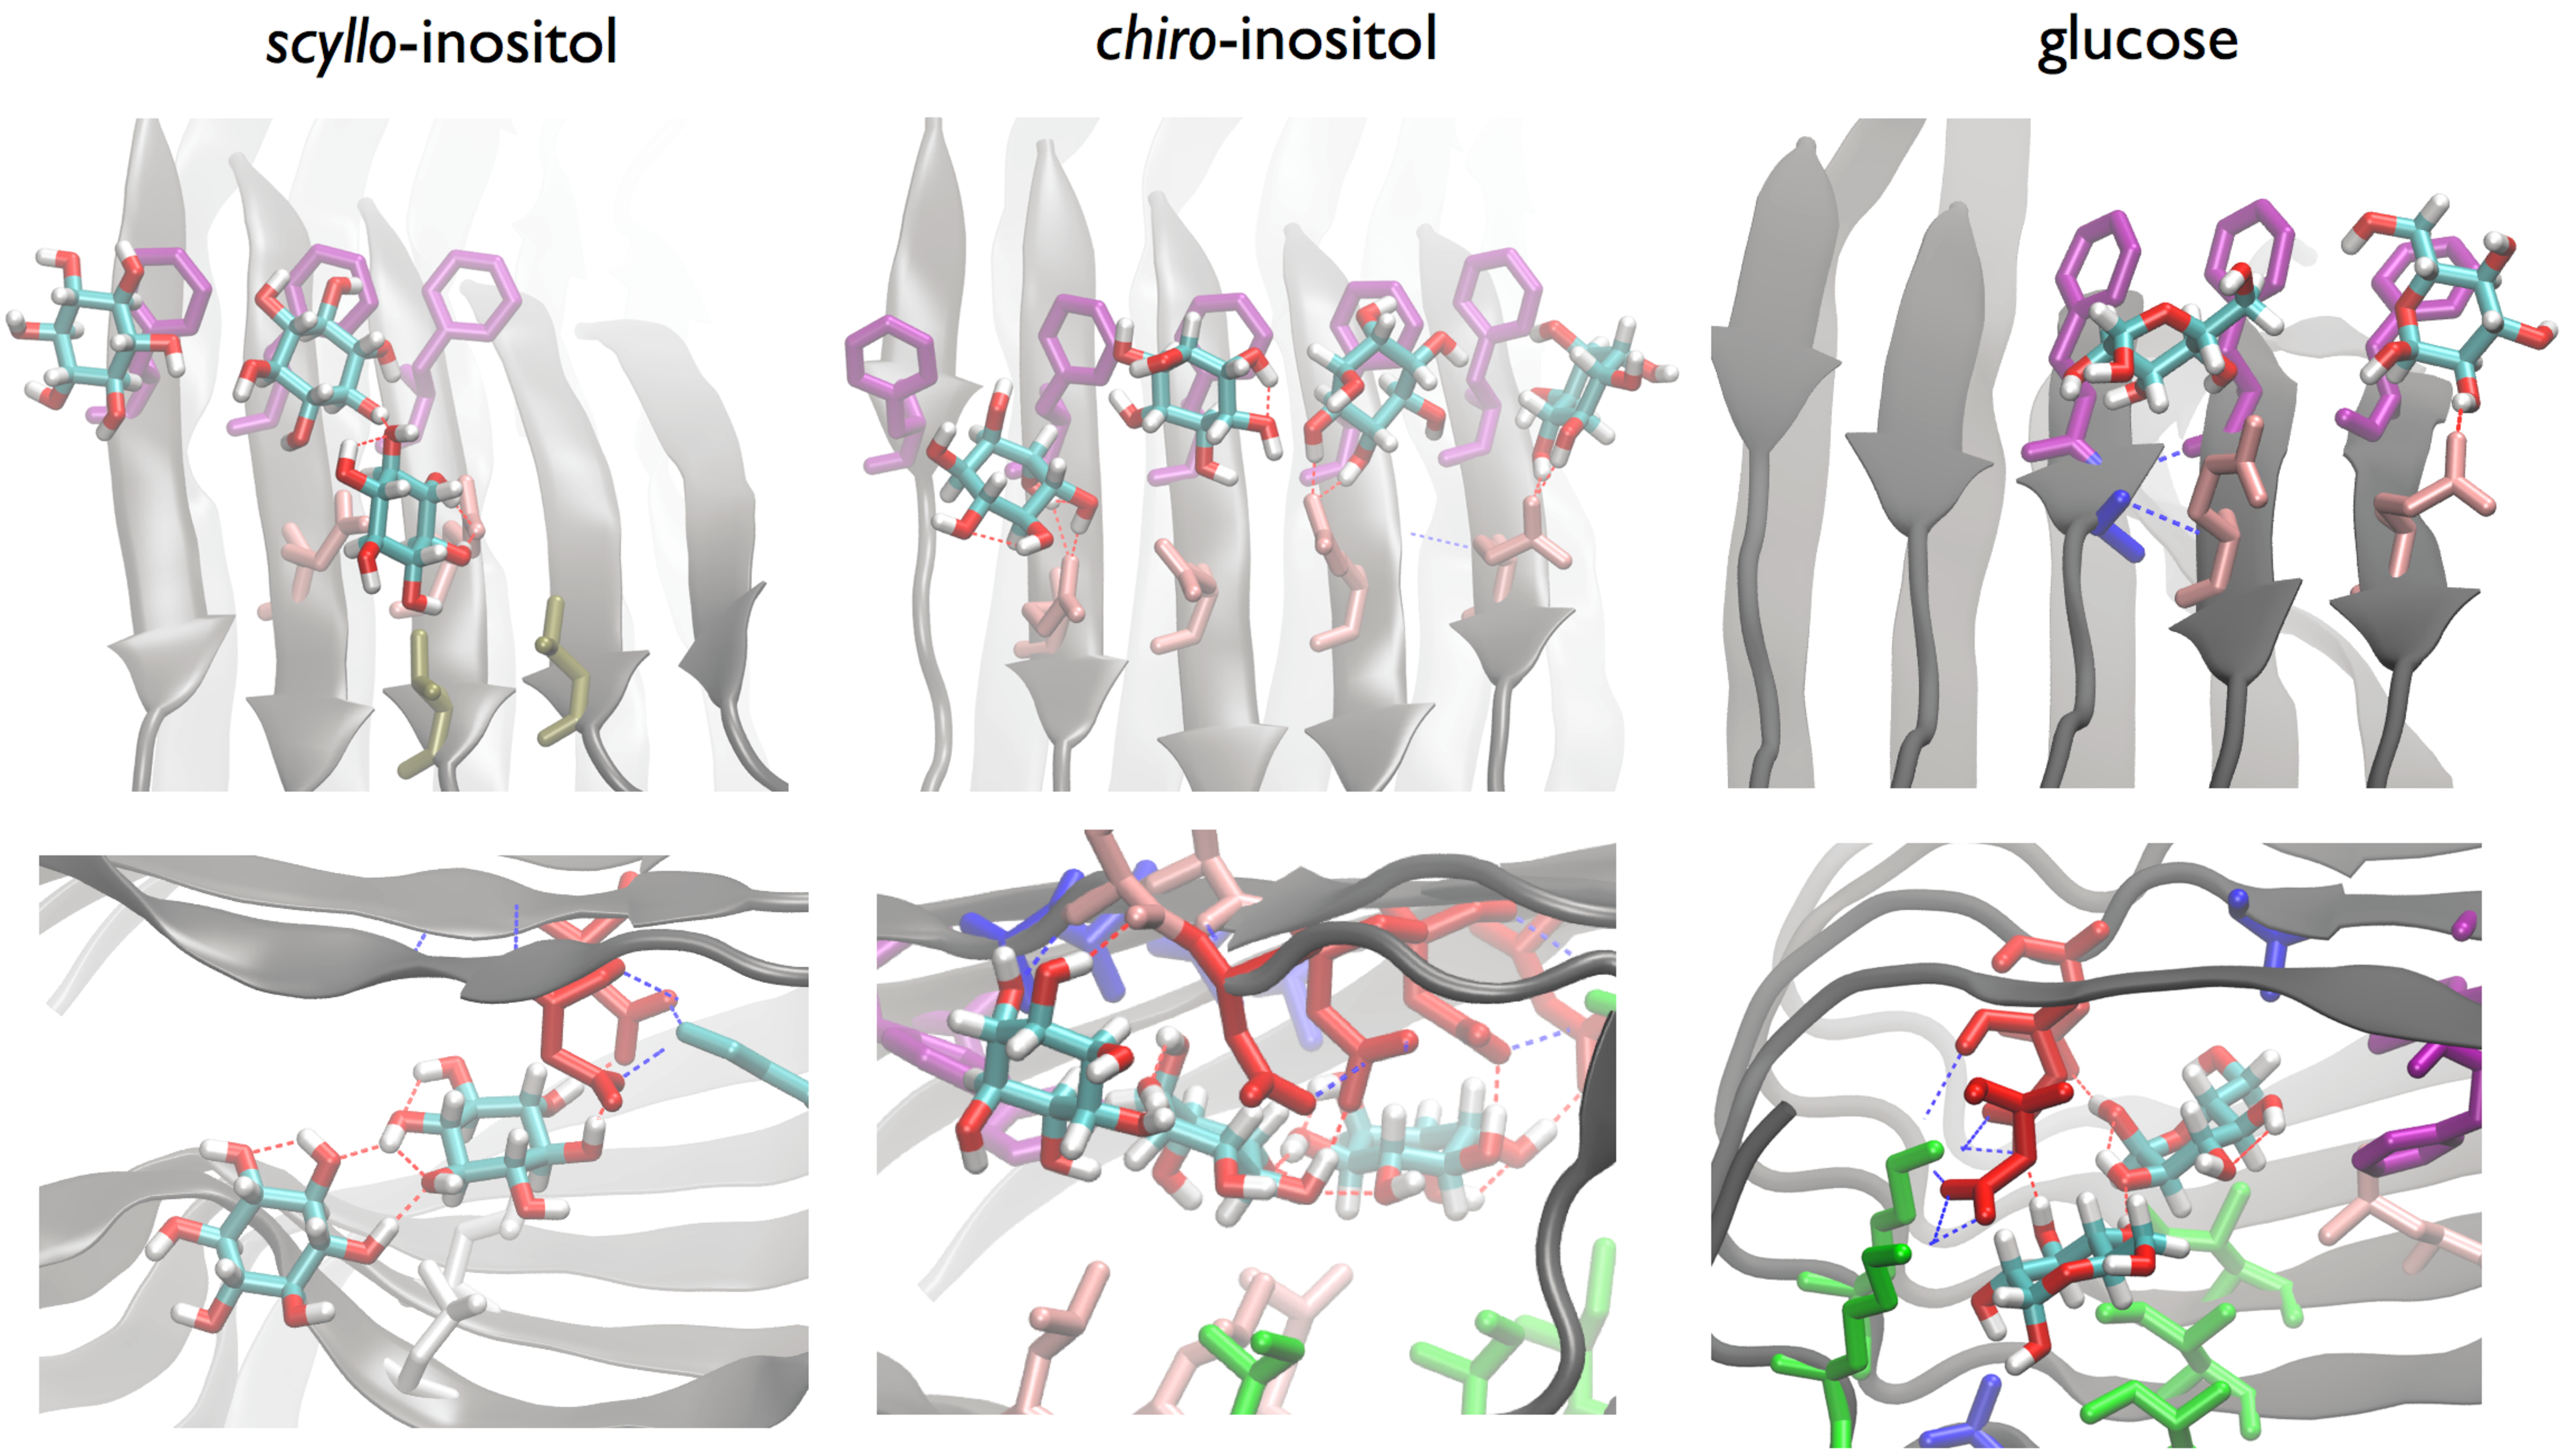
\includegraphics[width=6.5in]{figures/results3/detailed_binding_modes.pdf}
 \caption[Example binding modes of \textit{scyllo}-inositol, \textit{chiro}-inositol, and glucose to the protofibril]{Binding modes of \textit{scyllo}-inositol, \textit{chiro}-inositol and glucose to the $\beta$1 face (top row) and channel-like groove (bottom row). Residues that are within 4 \angstrom\ of a bound solute are represented in stick form. Protein is represented as a cartoon in gray.  Residues Phe, Glu, Asp, Lys and Ile are shown in purple, pink, red, green, and light green, respectively.}
 \label{fig:detailed_binding_modes}
\end{figure}

In addition to partitioning to different binding sites, both ligand binding modes and propensities also were modulated by ligand stereochemistry. In particular, \textit{scyllo}-inositol has the highest percentage of molecules bound exclusively via hydrogen bonding ($\sim$26\%).  Furthermore, only \textit{scyllo}-inositol molecules formed nonpolar contacts (24\%) and hydrogen bonds (26\%) with the fibril in approximately equal proportions (Figure~\ref{fig:spatial_binding}). By contrast, a higher fraction of \textit{chiro}-inositol, glucose, and glycerol molecules binding involved nonpolar contacts (Figure~\ref{fig:spatial_binding}). Furthermore, the fraction of molecules bound by exclusively nonpolar contacts increased concomitantly with a decrease in the fraction bound by exclusively hydrogen bonds in the following order: \textit{scyllo}-inositol (26\%, 22\%), \textit{chiro}-inositol (33\%, 13\%), glucose (37\%, 9\%), and glycerol (50\%, 11\%) (Figure~\ref{fig:spatial_binding}). \textit{Scyllo}-inositol with its planar hydrophobic faces and all-equatorial hydroxyl groups, has the stereochemistry most prone to  form hydrogen bonds with the protofibril.  The loss of planar nonpolar faces in \textit{chiro}-inositol reduced the hydrogen-bonded-only population by $\sim$9\%. Glucose, with one less hydroxyl group than the inositol stereoisomers, saw a 13\% reduction in the population bound by exclusively via hydrogen bonds.  Glycerol, which lacks a carbon ring and has the smallest number of hydroxyl groups, was most likely to interact via non-specific nonpolar contacts. Corroborating the results of our previous study,\cite{Li:2013fo} the results of this study suggest that the ability to form both hydrogen bonds and nonpolar contacts equally favorably is an important property of small molecules (to target the CHC) and therefore, ultimately, for the inhibition of amyloid formation.
% Elaborate -- what are the implications of this finding?  Are there current papers which suggests this?  In my inos2 paper, I mentioned this and RP mentioned that this is really what is coming out of this study. Maybe discuss this in more detail than what was covered in inos2 ...
% Discuss the trend where scyllo, chiro, glucose, and glycerol have increasing nonpolar-only contacts and decreasing polar only contacts, but nonpolar and polar remained relatively stable.

% Our previous study indicated that the balance of nonpolar and hydrogen bonding interactions is important (and dictates the binding specificity!!!) in inositol binding to monomer and aggregates of the peptide KLVFFAE because that is where scyllo and chiro differed in their binding modes.
% Solutes were also found to bind to the residues located in the turn region (on the surface). This and binding inside the tunnel are binding modes that are unlikely to be involved in amyloid inhibition.

\begin{figure}[htbp]
  \centering
  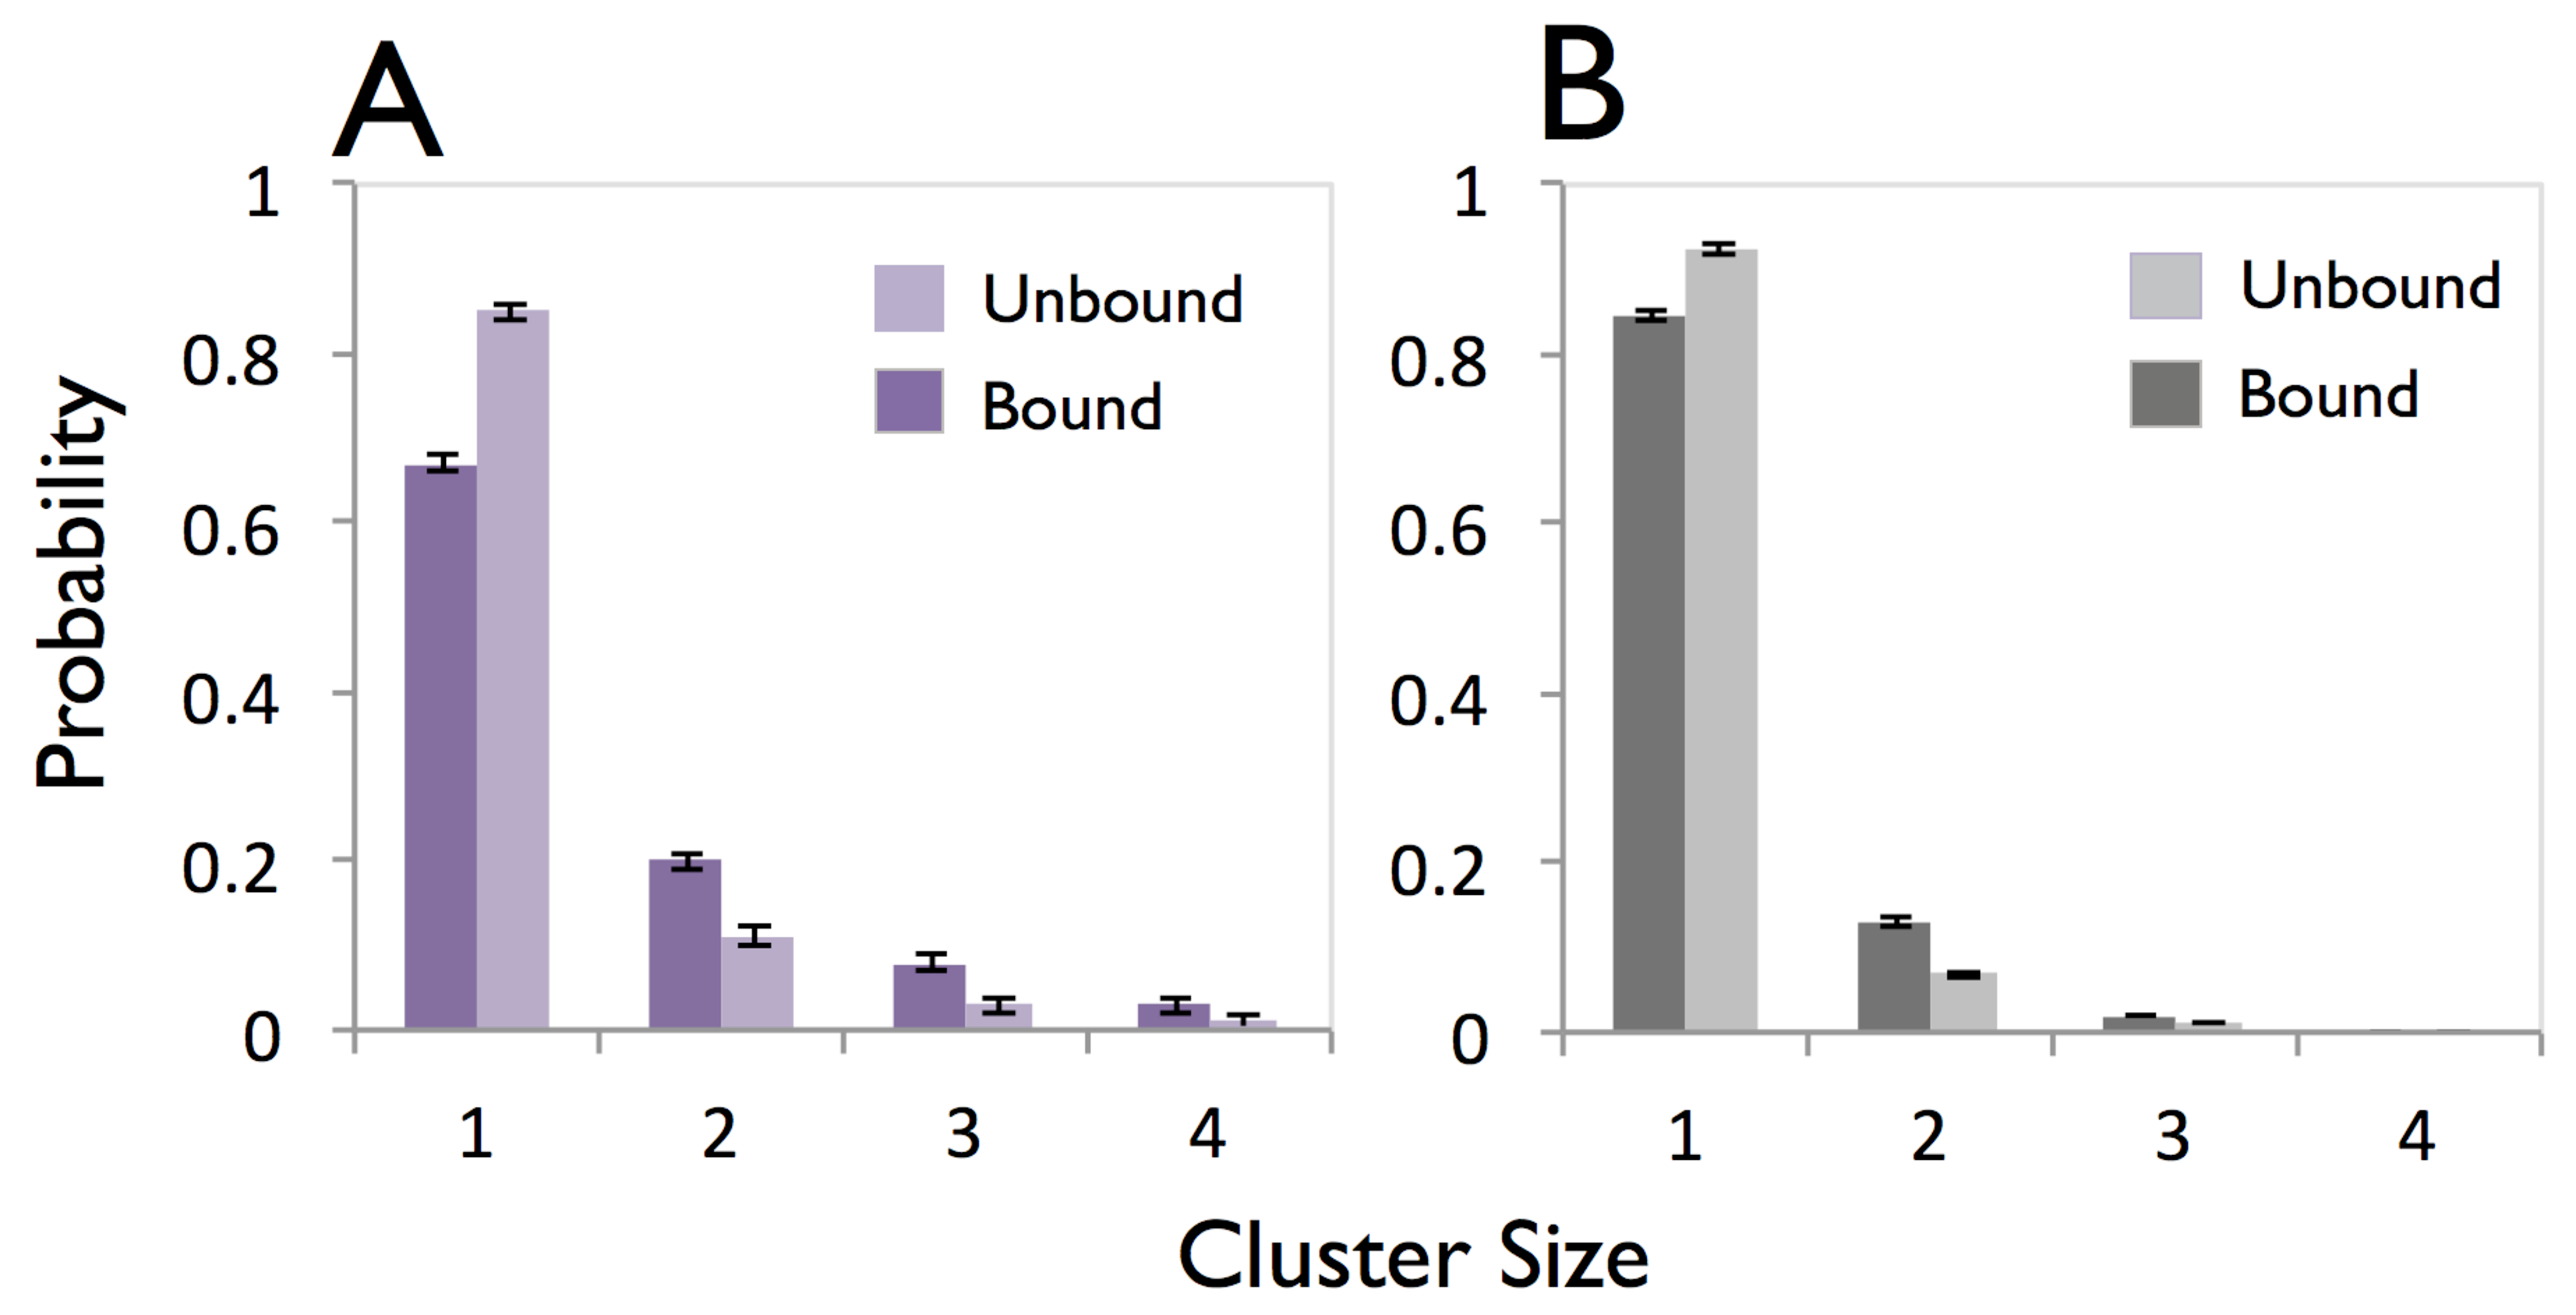
\includegraphics[width=6in]{figures/results3/clustered_binding.pdf}
  \caption[Clustered binding of solutes at the surface of the protofibril]{Probability distribution of bound vs. unbound cluster sizes for (A) \textit{scyllo}-inositol and (B) glycerol.}
  \label{fig:cluster_binding}
\end{figure}

Another important aspect of binding is the ability to bind in clusters (Figures~\ref{fig:detailed_binding_modes},\ref{fig:cluster_binding}). \textit{Scyllo}-, \textit{chiro}-inositol, and glucose each bound to the protofibril in a supermolecular form with no difference in their cluster size distributions (Figure~\ref{fig:cluster_binding}). By contrast, the distribution of cluster sizes for glycerol indicates that it is less likely than the other ligands to form clusters when bound.  Ligand molecules within a cluster form self-interactions via intermolecular hydrogen bonds and nonpolar contacts. Examples of such binding modes are shown in Figure~\ref{fig:detailed_binding_modes}.

Our previous study on the binding mechanism of inositol with the protofibril of A$\beta$(16-22)\cite{Li:2013fo} suggested that the ability of inositol to bind in clusters is a mechanism by which to increase the local concentration of bound ligands at the surface. Our result here is consistent with that study and we speculate that clustered binding modes of small molecules also play a role in the amyloid inhibition of full-length A$\beta$.  In support of these results, amyloid dye molecules in recent simulations\cite{Shea:2012eh} and Congo red in experiments,\cite{Stopa:2003wy} were also observed to adopt similar binding modes.

\subsection{Molecular basis of amyloid inhibition by \textit{scyllo}-inositol}
% \section{Discussion}
% - Binding specificity of inositol
%  - mention binding to FAE - but why?; should have a discussion of amyloid inhibition based on the observed binding modes;
% -  discussion of how the full length binding compares with KLVFFAE binding - impt mention that the binding modes are consistent in all models - comforting result

% Comment on MD simulations as a technique as a whole for understanding these types of interactions -- should this be a discussion point? -- maybe move this to conclusions  

Experimental evidence suggests that residues 17 to 21 (LVFFA) forming the central hydrophobic core of full-length A$\beta$ peptide are responsible for the initiation of A$\beta$ aggregation and $\beta$-sheet formation.\cite{deGroot:2006p4453}  Our study in chapter 3 indicated that the likely mode of action of inositol is to bind to exposed surfaces of $\beta$-sheets of A$\beta$(16-22).\cite{Li:2013fo} 
% Both Joanne and Mark said tonnes of literature supporting this face is relevant for inhibition!!!  --- where is this literature?
% Thus far, our results suggest that  scyllo best (or rather more specifically) to this face. This is an interesting conclusion / difference that thus only could tell from from the abeta42 model because it has two different faces which brought out the preferential binding of scyllo to the KLVFFAE face.
% Taken together, our results suggest that selectively targeting the CHC \textbf{is a good approach for developing potential amyloid inhibitors}.
% Scyllo- binds this face better than chiro-, glucose, and glycerol inactive solutes in fibril inhibition.  
% We speculate (is it speculation?) that the activity of scyllo-inositol in the inhibition of fibril formation is due to its preference for binding to the $\beta$-sheet face of the protofibril involving the residues in the CHC of \ab42. 
% Furthermore, we speculate that scyllo-inositol is active because it adopts more inhibition-productive binding modes than both chiro-inositol and glucose. Consistent with these results, our previous studies have indicated that scyllo-inositol binds with higher specificity with nonpolar groups of A$\beta$(16-22) than chiro-inositol. \textbf{For example, when chiro-inositol binds inside of the channel is a ``non-productive'' binding modes.} - Not sure if any of these are based on any results.
The spatial binding probability distributions, depicted in Figure~\ref{fig:spatial_binding}, indicate that \textit{scyllo}-inositol has the highest preference for the face of the protofibril containing the residues found in the central hydrophobic core (CHC) of A$\beta$, particularly to the groove formed by the residues F-A-E. By contrast, the inactive molecules, \textit{chiro}-inositol and glucose, were both found to predominantly partition to the $\beta$2 face, taking part in nonspecific binding. This result is in accordance with our previous study (Chapter 4)\cite{Li:2013fo} where we showed that \textit{scyllo}-inositol displays higher binding specificity to phenylalanine: \textit{scyllo}-, unlike \textit{chiro}-inositol, adopts a face-to-face binding mode with phenylalanine. By contrast, due to stereochemistry differences, \textit{chiro}-inositol and glucose molecules do not possess such a binding mode. Consistent with this result, both \textit{chiro}-inositol and glucose displayed less binding specificity for the CHC and were predominantly bound via nonspecific nonpolar contacts.
 
On the basis of our results, we hypothesize that the CHC, particularly residues Phe20 and Glu21, is a critical binding site of \textit{scyllo}-inositol for preventing the formation of A$\beta$42 fibrils. \textit{Scyllo}-inositol, unlike \textit{chiro}-inositol, is able to inhibit fibril formation due to its binding specificity for the amyloidogenic core of A$\beta$42.  Our results support the hypothesis that selectively targeting the CHC segment of the A$\beta$ may be a viable approach for the inhibition of A$\beta$ fibrillation. 

This binding specificity of an in vitro small molecule inhibitor is modulated by both the stereochemistry of the small molecule and physicochemical properties of the fibril surface that is available for binding.  For example, similar to \textit{scyllo}-inositol, anthraquinone was also suggested to act by binding to residues LVFFA in a recent simulation study by Convertino \textit{et al.}\cite{Convertino:2011epa}  By contrast, the polyphenol morin, a predominantly hydrophobic compound,  was found to not interact with residues in the CHC, but rather bound to residues at the C-terminal end of the protofibril.\cite{Lemkul:2010bf}
% Their binding is less specific to the same region than that of scyllo-inositol.  
% Taken together, our results indicate that the binding specificity of scyllo-inositol is to the amyloidogenic core of A$\beta$ amyloid. This is consistent with what we found in our KLVFFAE study.

% On the basis of our results, we hypothesize that binding to the face of protofibrils containing the residues LVFFAE may be a productive small-molecule binding mode for the inhibition of lateral stacking of fibrils.  The difference in the binding specificity of scyllo- and chiro-inositol towards the $\beta$1 face may explain the differences between the activity of scyllo- and chiro-inositol in the inhibition of A$\beta$ amyloid fibrillation.  
Because of its binding specificity, \textit{scyllo}-inositol may prevent the lateral association of fibrillar aggregates by binding to the $\beta$1 face, which has been suggested to be involved in the lateral stacking of protofilaments which ultimately become mature amyloid fibrils. Without the ability to stabilize the cross-$\beta$ structure by stacking laterally, single-layered protofibrillar structures are� unlikely to propagate into mature fibrils. 
%which ultimately lead to inhibition of amyloid formation.. % ie. require stacking to grow into the long unbranched morphology seen in EM.

\subsection{Comparisons of binding to the protofibril of A$\beta$(16-22)}
% \textbf{Have a paragraph discussing the consistency of results here and the results in my previous studies.  I'm being too repetitive if I mention that it's consistent with KLVFFAE after every results and discussion paragraph}
% Comment on how good are these model peptides for understanding inhibitor binding interactions. Do I really want to discuss this? I think this is better to discuss in my thesis conclusions?
% Depending on the morphology of the amyloidogenic aggregate, the binding modes can be different. 
In a previous study (see Chapter 3), we investigated the binding mechanism of inositol stereoisomers with protofibrillar oligomers of A$\beta$(16-22).\cite{Li:2013fo} Unlike A$\beta$42, the protofibril of A$\beta$(16-22) presents two chemically identical faces consisting of the same polar, charged and hydrophobic grooves. For this reason, in that study, \textit{scyllo}-inositol and \textit{chiro}-inositol were found to bind in similar binding sites protofibril of A$\beta$(16-22). Although binding modes of a small molecule may remain consistent across amyloid morphologies of different peptide sequences, its binding site and binding specificity can be modulated by the fibril surface properties. As a consequence, comparatively examining the binding modes of several small molecules with differing activities is crucial for determining the molecular mechanism of a small molecule amyloid inhibitor.

Taken together, our study suggests that examining binding to model amyloidogenic peptides is useful for eliminating the large number of possible binding modes and binding sites associated with amyloid inhibitors. However, because the activity of small-molecule inhibitors is specific to both sequence and morphology, it is necessary to ultimately examine their binding with the fibrillar aggregate of the full-length A$\beta$.

% The core of the abeta42 fibril solved by Luhrs et al. protofibril of the Abeta42 can be thought of as an early beta-sheet oligomer of Abeta42. 
% Binding modes with aggregates of model abeta peptides may have modes that differ from the full length amyloid. 
%It may have been that for this reason, we observed that both scyllo and chiro were bound with similar Keq to the protofibril of KLVFFAE.  
% However, with differing faces on the Abeta protofibril, we were  able to identify preferential binding of scyllo- to the KLVFFAE face.

% We speculate that becauseF scyllo-inositol is not trapped by unproductive binding modes, this may explain why scyllo-, but not chiro-inositol, is active in the inhibition of \ab42. - Not so sure about this idea.

% \textbf{The discussion of why not Abeta40 but Abeta42 should be included at the end of the discussion section as this is going to be quite speculative - it may be because of differing binding modes due to differences in fibril structure}. However, further studies that are similar to the current study will be needed to elucidate differences in their binding. 

% First study where we comparatively examine a small molecule inhibitor ?
% Our results not only suggests mechanism by which scylllo inhibits but also reveals why small molecules don?t ?work?. 

% In addition to stereochemistry-dependent activity, inositol was found to be inactive for inhibiting the amyloid formation of Abeta40 - put forth a few speculations based on the data of my current study to explain.  

% \textbf{More speculative - Relevance of the NMR models.} I can say something about the suggested accuracy of the NMR models based on my sim. results?  Radius of gyration? The model falls apart? Does this mean that the NMR model is not ``right'' ? Is the pentamer a stable unit of the fibril ? ``accuracy'' of the NMR models -- how good are these models?  It is unlikely I'm going to be able to say much here, we have no idea what the actual experimental stability of this species is.  This pentamer fragment may not be stable on its own, but could be just a building block in a stable extended fibrillar structure of A$\beta$42. -- But based on my recollection a study by Masman sugggests that this is the stable core. - I'm not sure if this is a useful thing to have in my discussion


% Whole idea:  binding at the surface and preventing stacking, rather than insertion.  Insertion is not likely to be a productive binding mode for inhibition. Why? because I don't observe disruptive insertion (I need to define this) - scyllo doesn't really insert, chiro- does, but no disruption to the aggregate ...
% More quantitatively I probably _need_ to quantify affinity to the KLVFFAE face of the Abeta fibril for scyllo chiro, glucose
% Also should do epi.  But what if epi does not bind to KLVFFAE face? How would I then explain that epi is also active but does not go to KLVFFAE? This could disprove my entire hypothesis ... though its not likely because chiro goes to the KLVFFAE face.
% I think a Shea paper talks about the importance of preventing stacking


\section{Conclusions}
In this study, we have performed extensive atomistic molecular dynamics simulations of \textit{scyllo}-inositol and its inactive stereoisomer, \textit{chiro}-inositol, and osmolytes glucose and glycerol, with the protofibril of the full-length A$\beta$42.  From our simulations, we characterized the stereochemistry-dependent ligand binding modes and their effect on the morphology of A$\beta$42 protofibrils.  Although no difference in the fibril conformation was found in the presence of thes ligands, stereospecific binding modes and binding sites were uncovered.  Most notably, \textit{scyllo}-inositol displays the highest binding specificity for residues in the central hydrophobic core of the fibrils of A$\beta$42, suggesting that small molecule inhibitors which target this region may be effective in preventing A$\beta$42 amyloid formation.
% No difference in the fibril conformations with and without inositol in either the low or high molar ratio simulations. Does glucose bind more or less? If it does bind less, then it tells us that we might be onto something with scyllo-inositol even though the structure is subtly different.  Glucose does not necessarily bind ``less", but it does not bind on the right face ie. the KLVFFAE face Scyllo-inositol appears to preferentially bind the KLVFFAE face, more than glucose and chiro-inositol.  Furthermore scyllo does not bind in a hydrated tunnel formed in the protofibrillar aggregate.  

%\section{Acknowledgements}
% We thank Drs. JoAnne McLaurin, Mark Nitz and Chris Neale for reading the manuscript and for providing insightful comments. 
%This work was made possible by the GPC supercomputer at the SciNet HPC Consortium and Compute/Calcul Canada (Colosse CLUMEQ). This work was supported in parts by the Canadian Institutes of Health Research (Grant No. MOP84496). R.P. is a CRCP chairholder.

% \section*{Supporting Information Available}
% Binding mode analyses of inositol with monomeric and aggregate systems at inositol concentrations and inositol:peptide molar ratios that were not shown in the main text; Analyses of peptide self-aggregation for the formation of the disordered oligomer; Snapshots of the starting simulation structure of the $\beta$-oligomer. Supporting Information Available: Full description of the material. This material is available free of charge via the Internet at http://pubs.acs.org.

%http://www.pnas.org/content/102/2/315.full
%Support for the Significance of the LVFFA binding:
% The central hydrophobic cluster of amyloid-β (residues 17–21 LVFFA) has been particularly implicated in amyloid fibril formation (19). Tjernberg et al. (20) found that the fragment QKLVFF binds to amyloid β to prevent amyloidogenesis, whereas follow-up studies investigated the short peptides, LVFFA (21) and LPFFD (22), and showed that they are also inhibitors and that the fragment KLVFFAE forms well ordered fibrils. 
%
%KLVFFA binds to ABeta42 -- do they where they bind?
%Tjernberg, L. O., Naslund, J., Lindqvist, F., Iohansson, J., Karlstrom, A. R., Thyberg, J., Terenius, L., and Nordstedt, C. (1996) Arrest of ������-amyloid fibril formation by a pentapeptide ligand, J. Biol. Chem. 271, 8545-8548.
%
%
%Second, Aβ(16-22) peptide, which includes the central HP core, CHC (LVFFA), is recognized as being essential for Aβ fibrillation (27,28) and also forms amyloid fibrils with antiparallel β-strands in isolation (29). Third, the KLVFF motif is a primary target in the search for aggregation inhibitors for AD therapeutics (30,31).
%28. Nilsberth C., Westlind-Danielsson A., Lannfelt L. The ‘Arctic’ APP mutation (E693G) causes Alzheimer's disease by enhanced Aβ protofibril formation. Nat. Neurosci. 2001;4:887–893. [PubMed]
%29. Balbach J.J., Ishii Y., Tycko R. Amyloid fibril formation by A β 16-22, a seven-residue fragment of the Alzheimer's β-amyloid peptide, and structural characterization by solid state NMR. Biochemistry. 2000;39:13748–13759. [PubMed]
%30. Lowe T.L., Strzelec A., Murphy R.M. Structure-function relationships for inhibitors of β-amyloid toxicity containing the recognition sequence KLVFF. Biochemistry. 2001;40:7882–7889. [PubMed]
%31. Lashuel H.A., Hartley D.M., Callaway D.J. New class of inhibitors of amyloid-β fibril formation. Implications for the mechanism of pathogenesis in Alzheimer's disease. J. Biol. Chem. 2002;277:42881–42890. [PubMed]
% \section*{Figures}

%\begin{figure}[htbp]
%  \centering
%  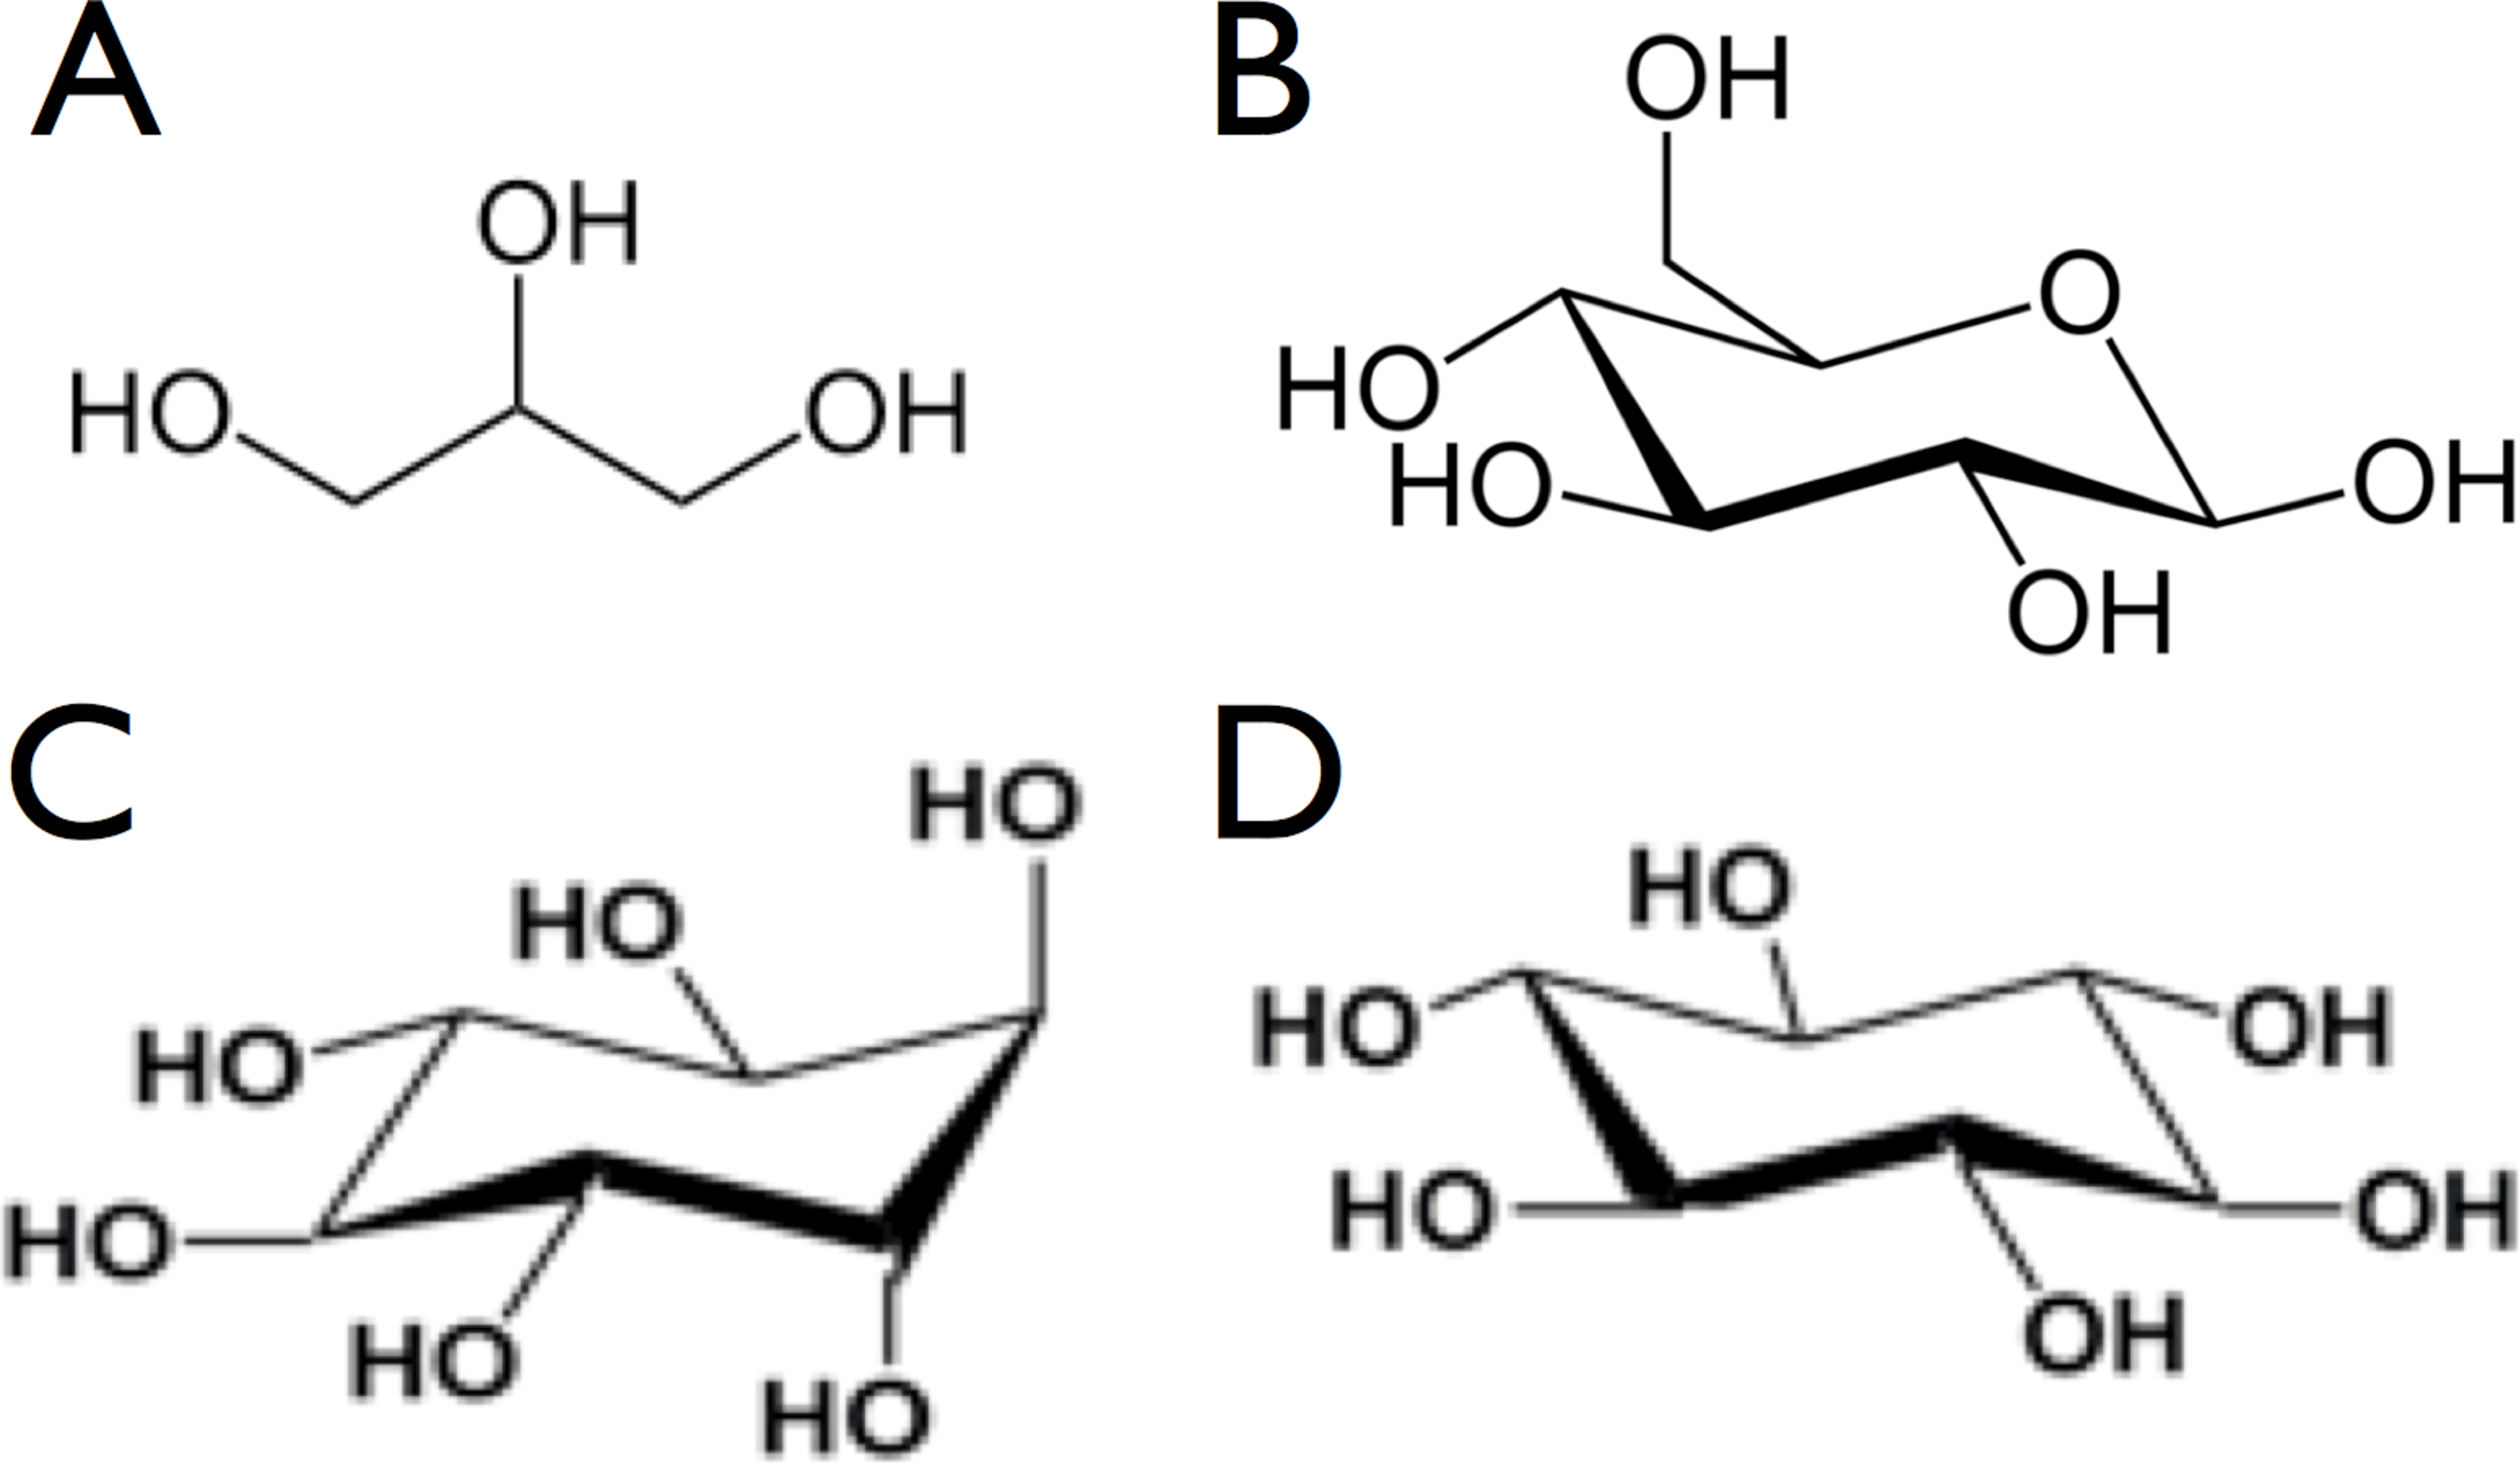
\includegraphics[width=2.5in]{figures/results3/ligands.pdf}
%  \caption[Ligands]{Molecular structures of (A) glycerol, (B) glucose, (C) chiro-inositol and (D) scyllo-inositol}
%  \label{fig:ligands}
%\end{figure}
%
%\begin{figure}[htbp]
%  \centering
%  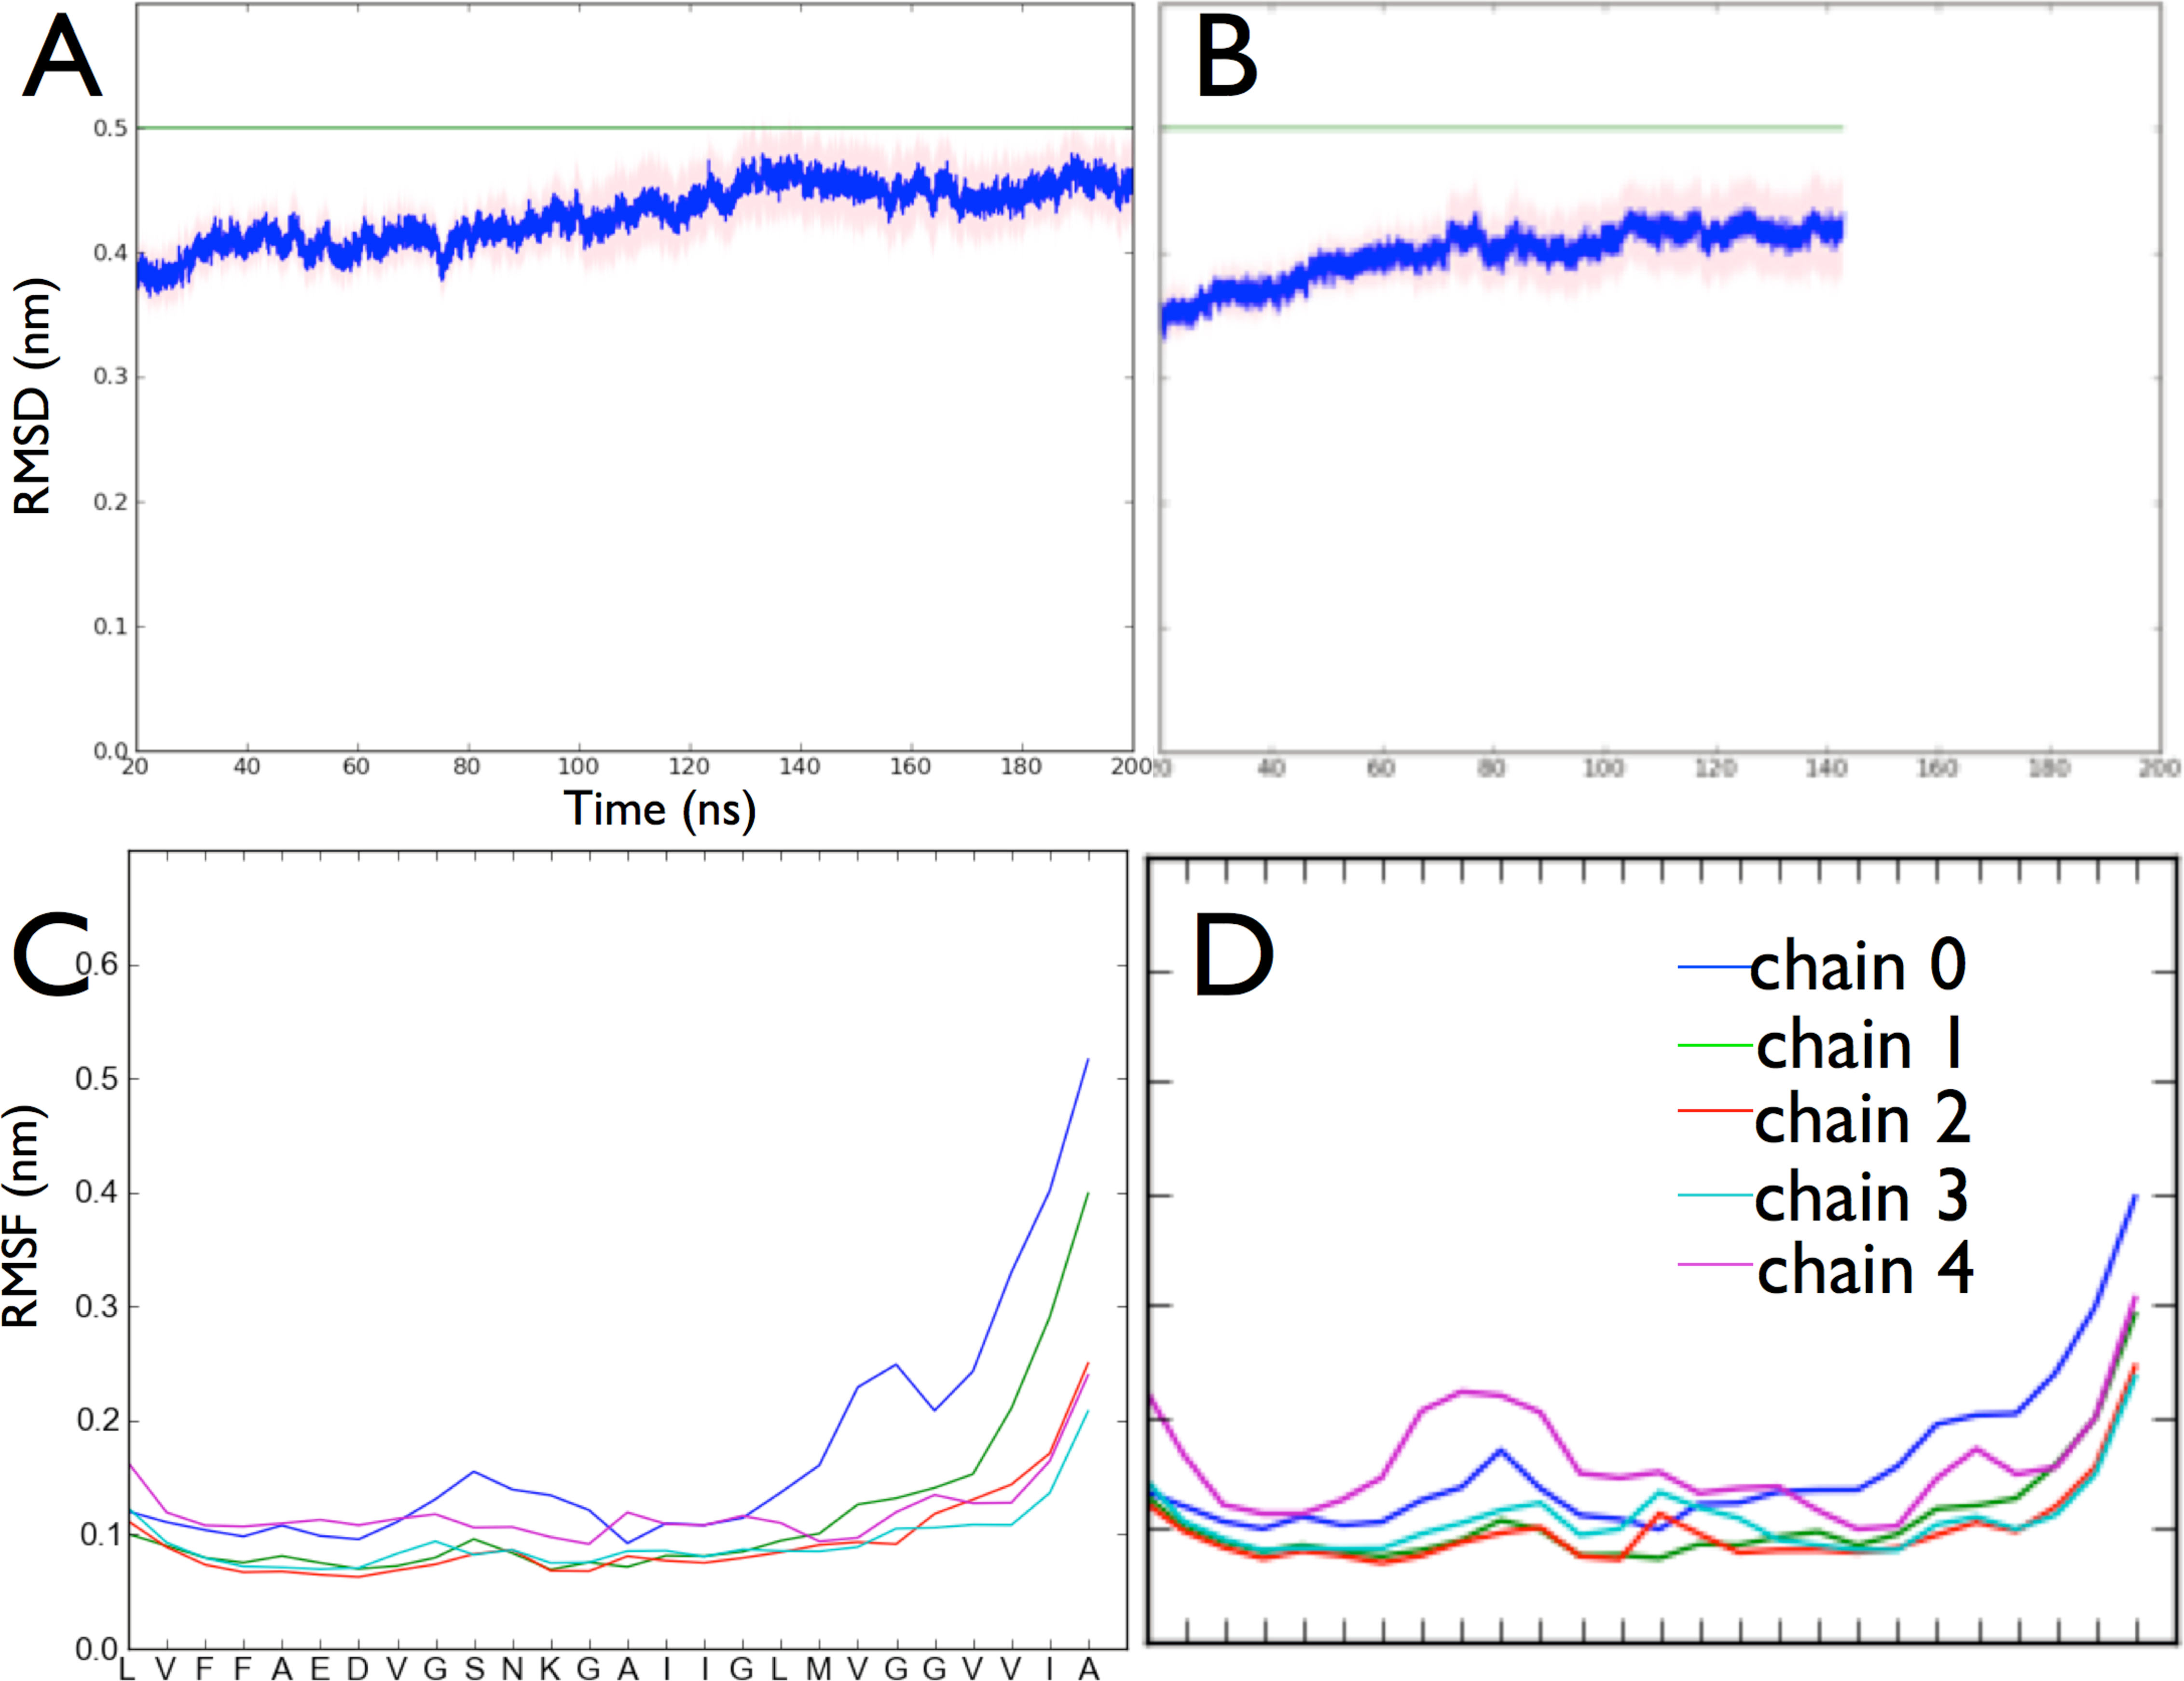
\includegraphics[width=5in]{figures/results3/protofibril_dynamics.pdf}
%  \caption[RMSD and RMSF vs. time]{Fibril structure dynamics in pure water (A) and (C), and in the presence of scyllo-inositol (B) and (D).}
%  \label{fig:protofibril_dynamics}
%\end{figure}

%\begin{figure}[htbp]
% \centering
 % 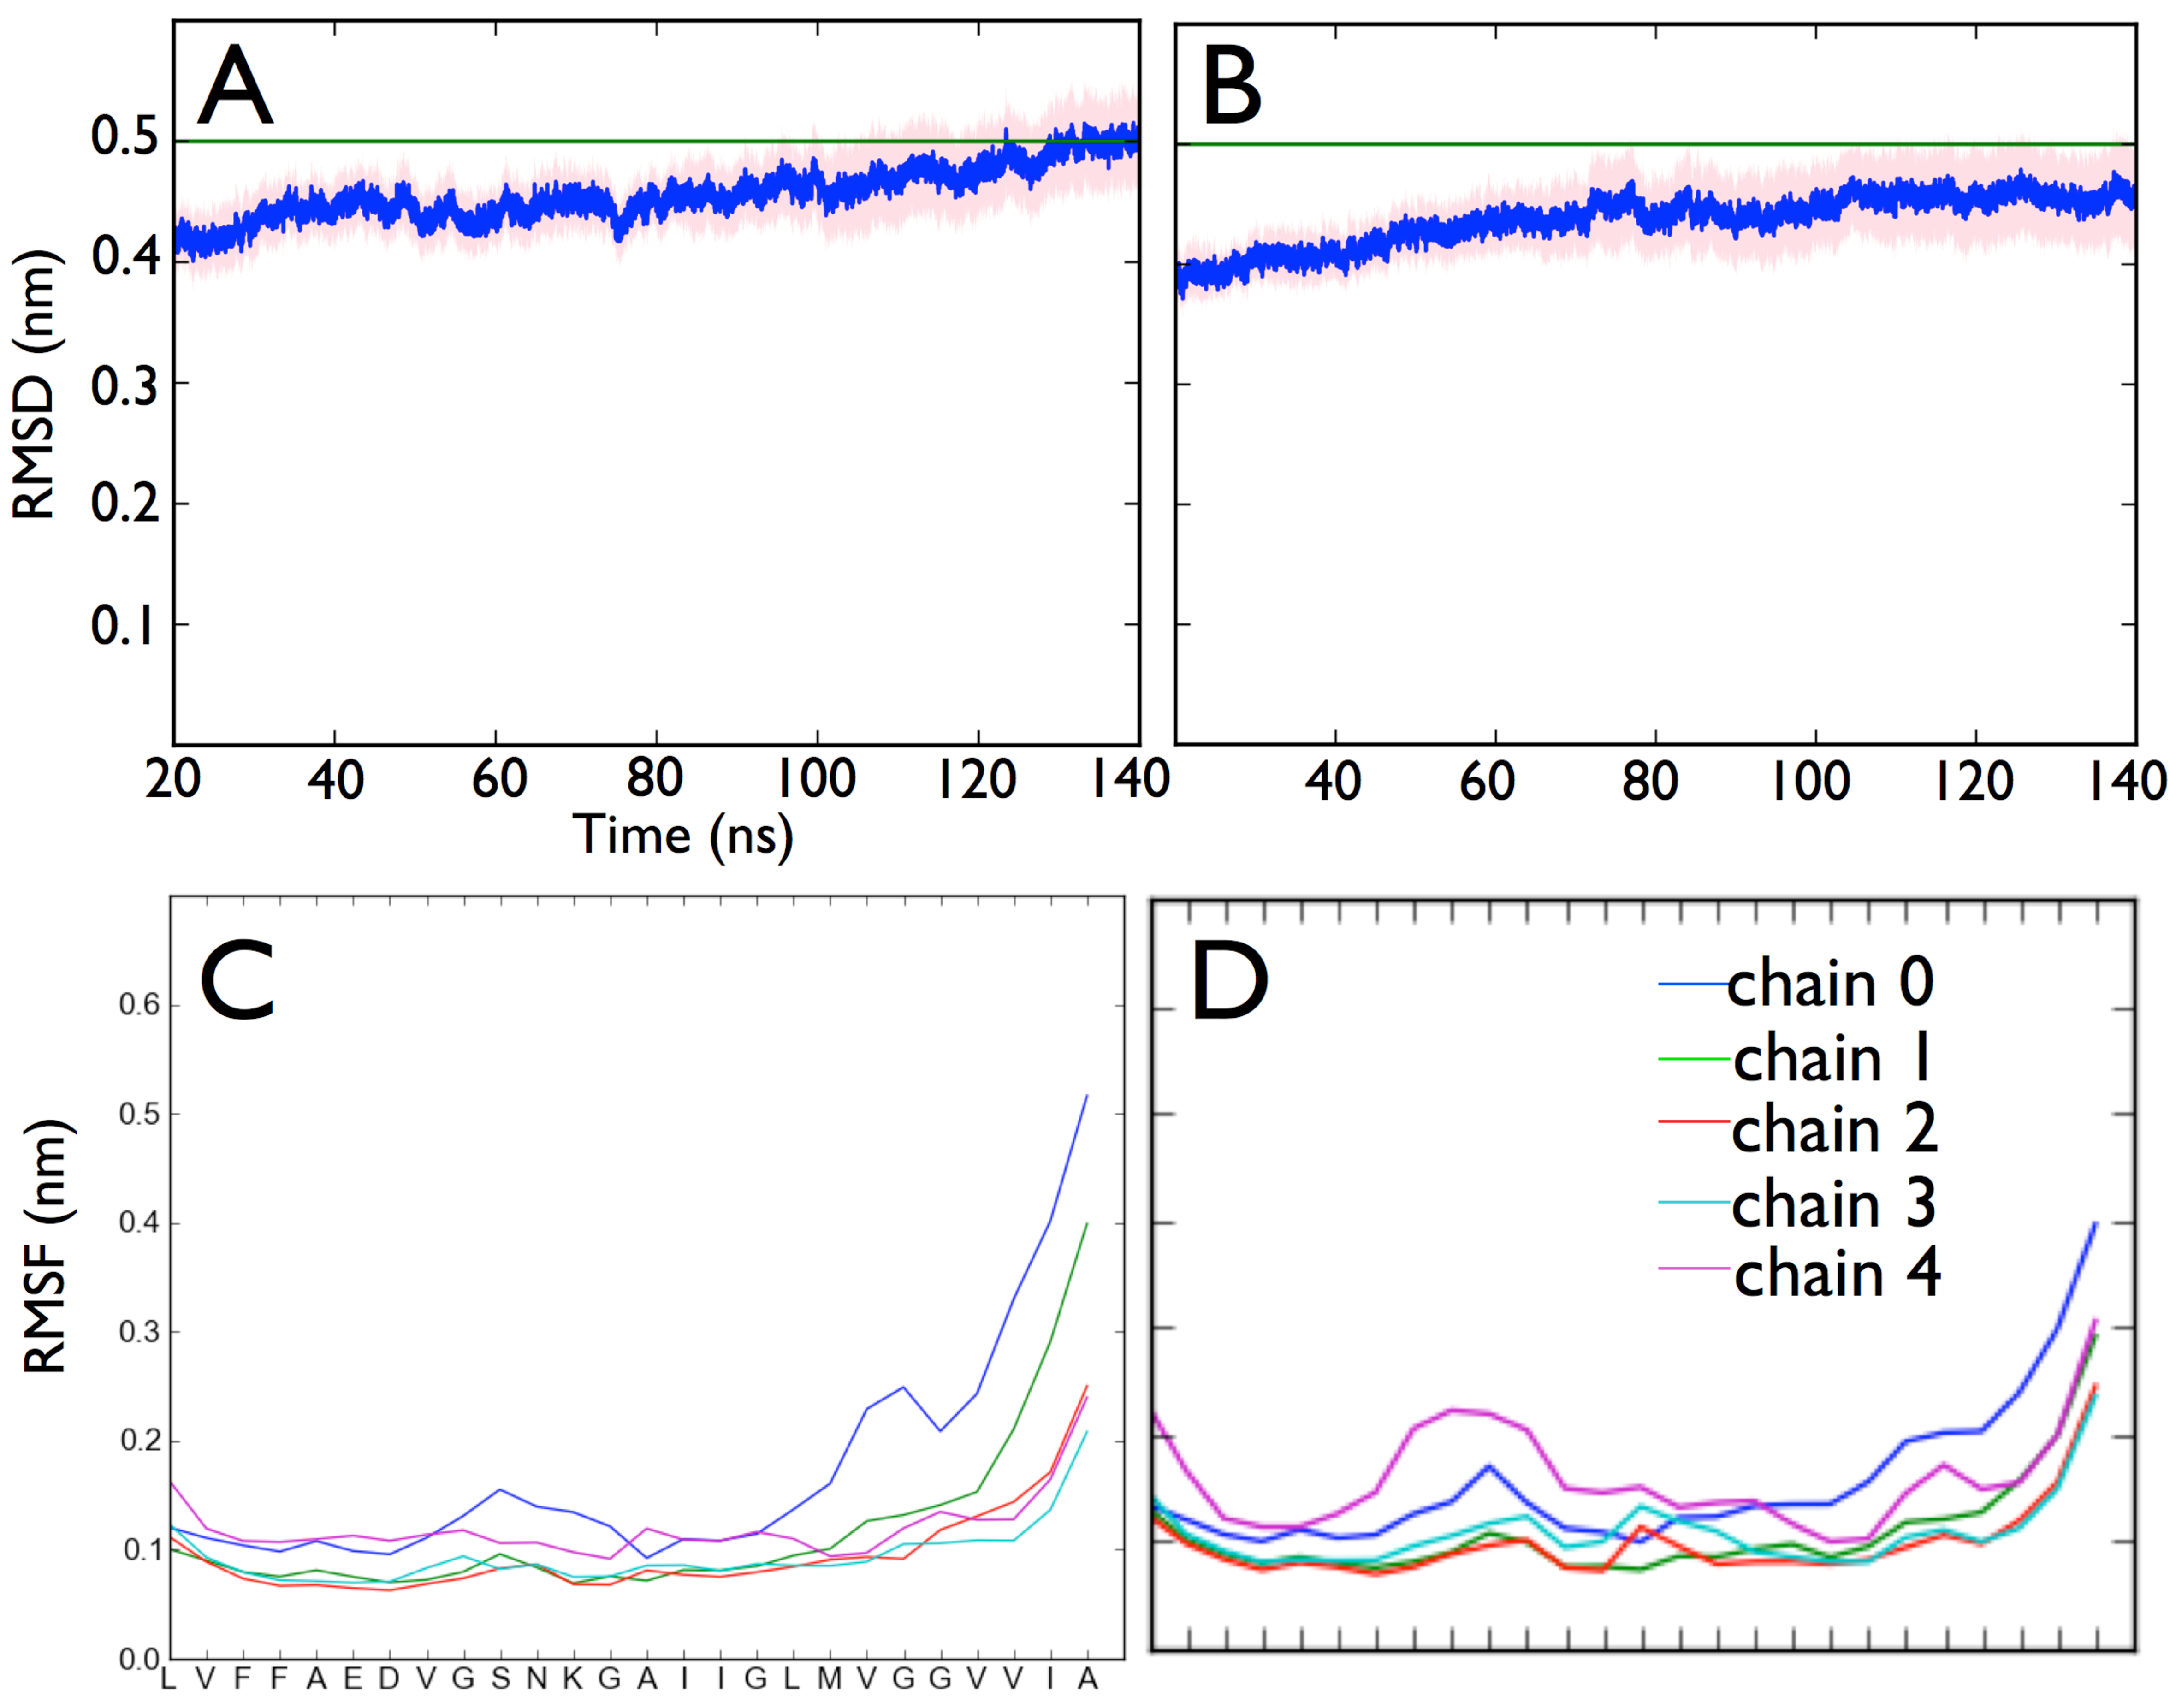
\includegraphics[width=5in]{figures/results3/protofibril_dynamics2.pdf}
% \caption[Secondary structure of protofibril]{(A) chain-chain (B) Secondary structure of fibril}
% \label{fig:protofibril_dynamics}
%\end{figure}

%\begin{figure}[htbp]
%  \centering
%  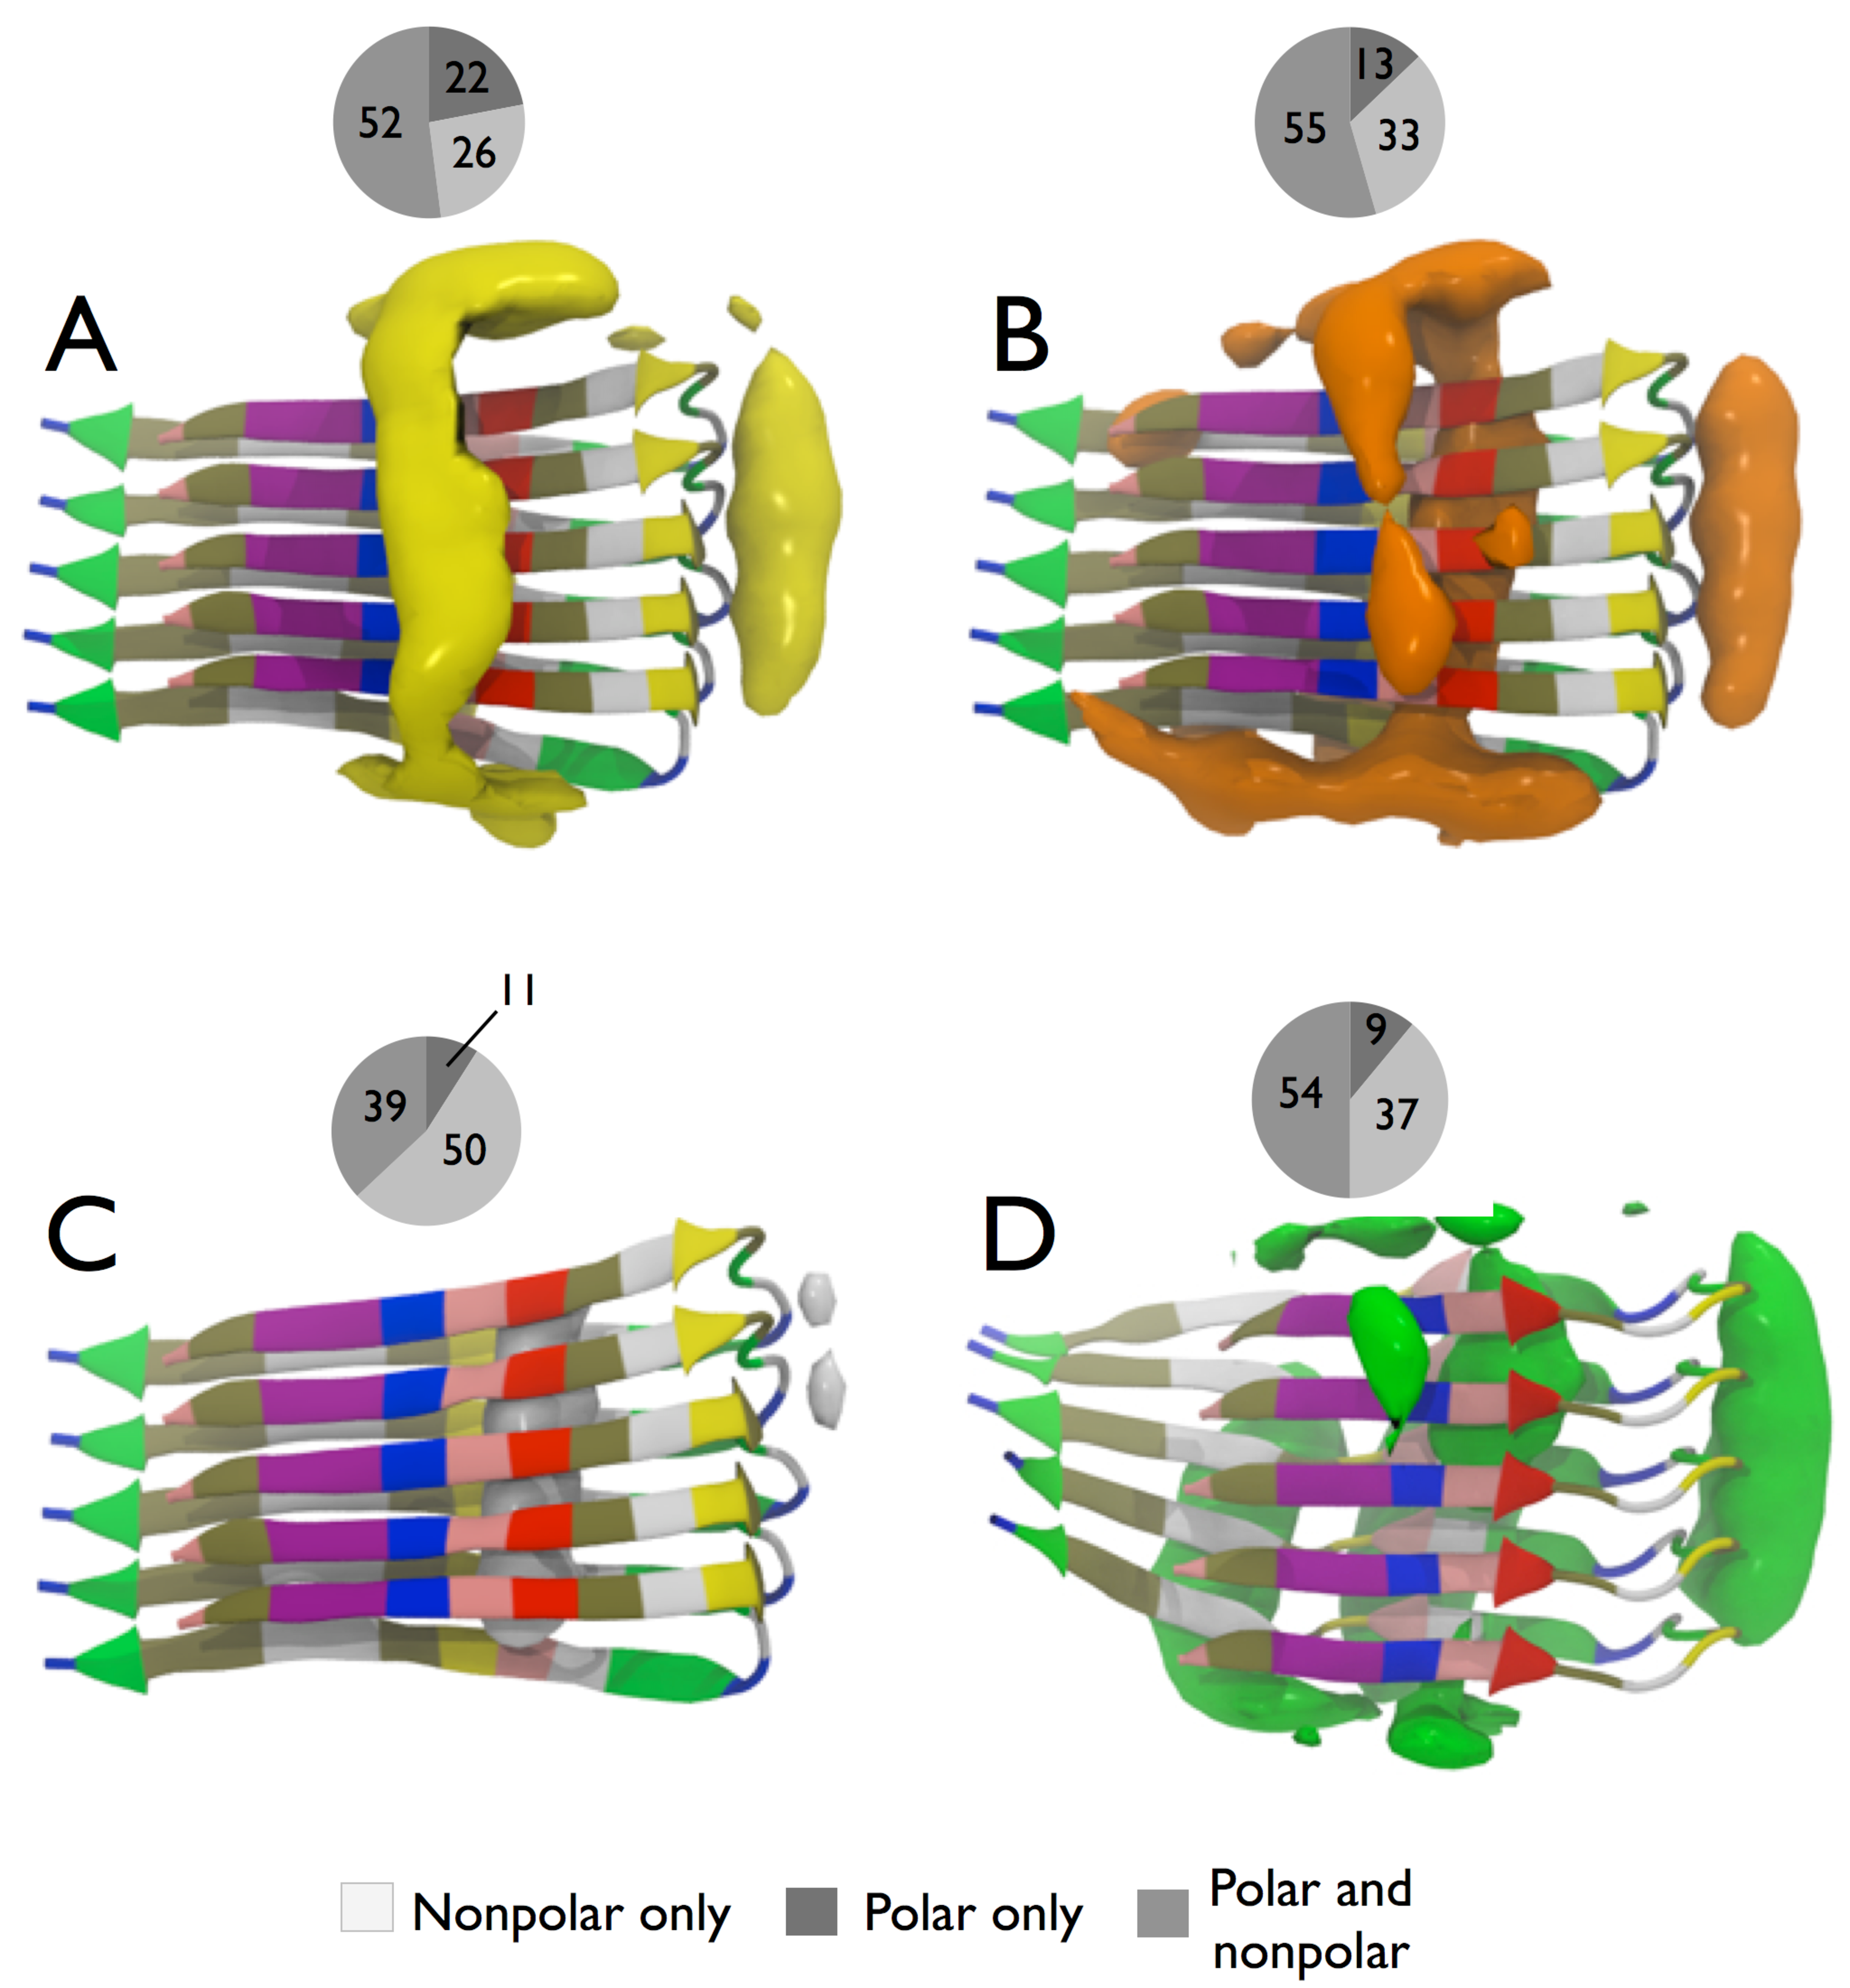
\includegraphics[width=6in]{figures/results3/binding_sdf_pie_chart.pdf}
%  \caption[Spatial probability distribution of bound solutes]{Comparisons of the spatial probability densities for (A) scyllo-inositol, (B) chiro-inositol (C) glycerol and (D) glucose.}
%  \label{fig:spatial_binding}
%\end{figure}

%\begin{figure}[htbp]
% \centering
% 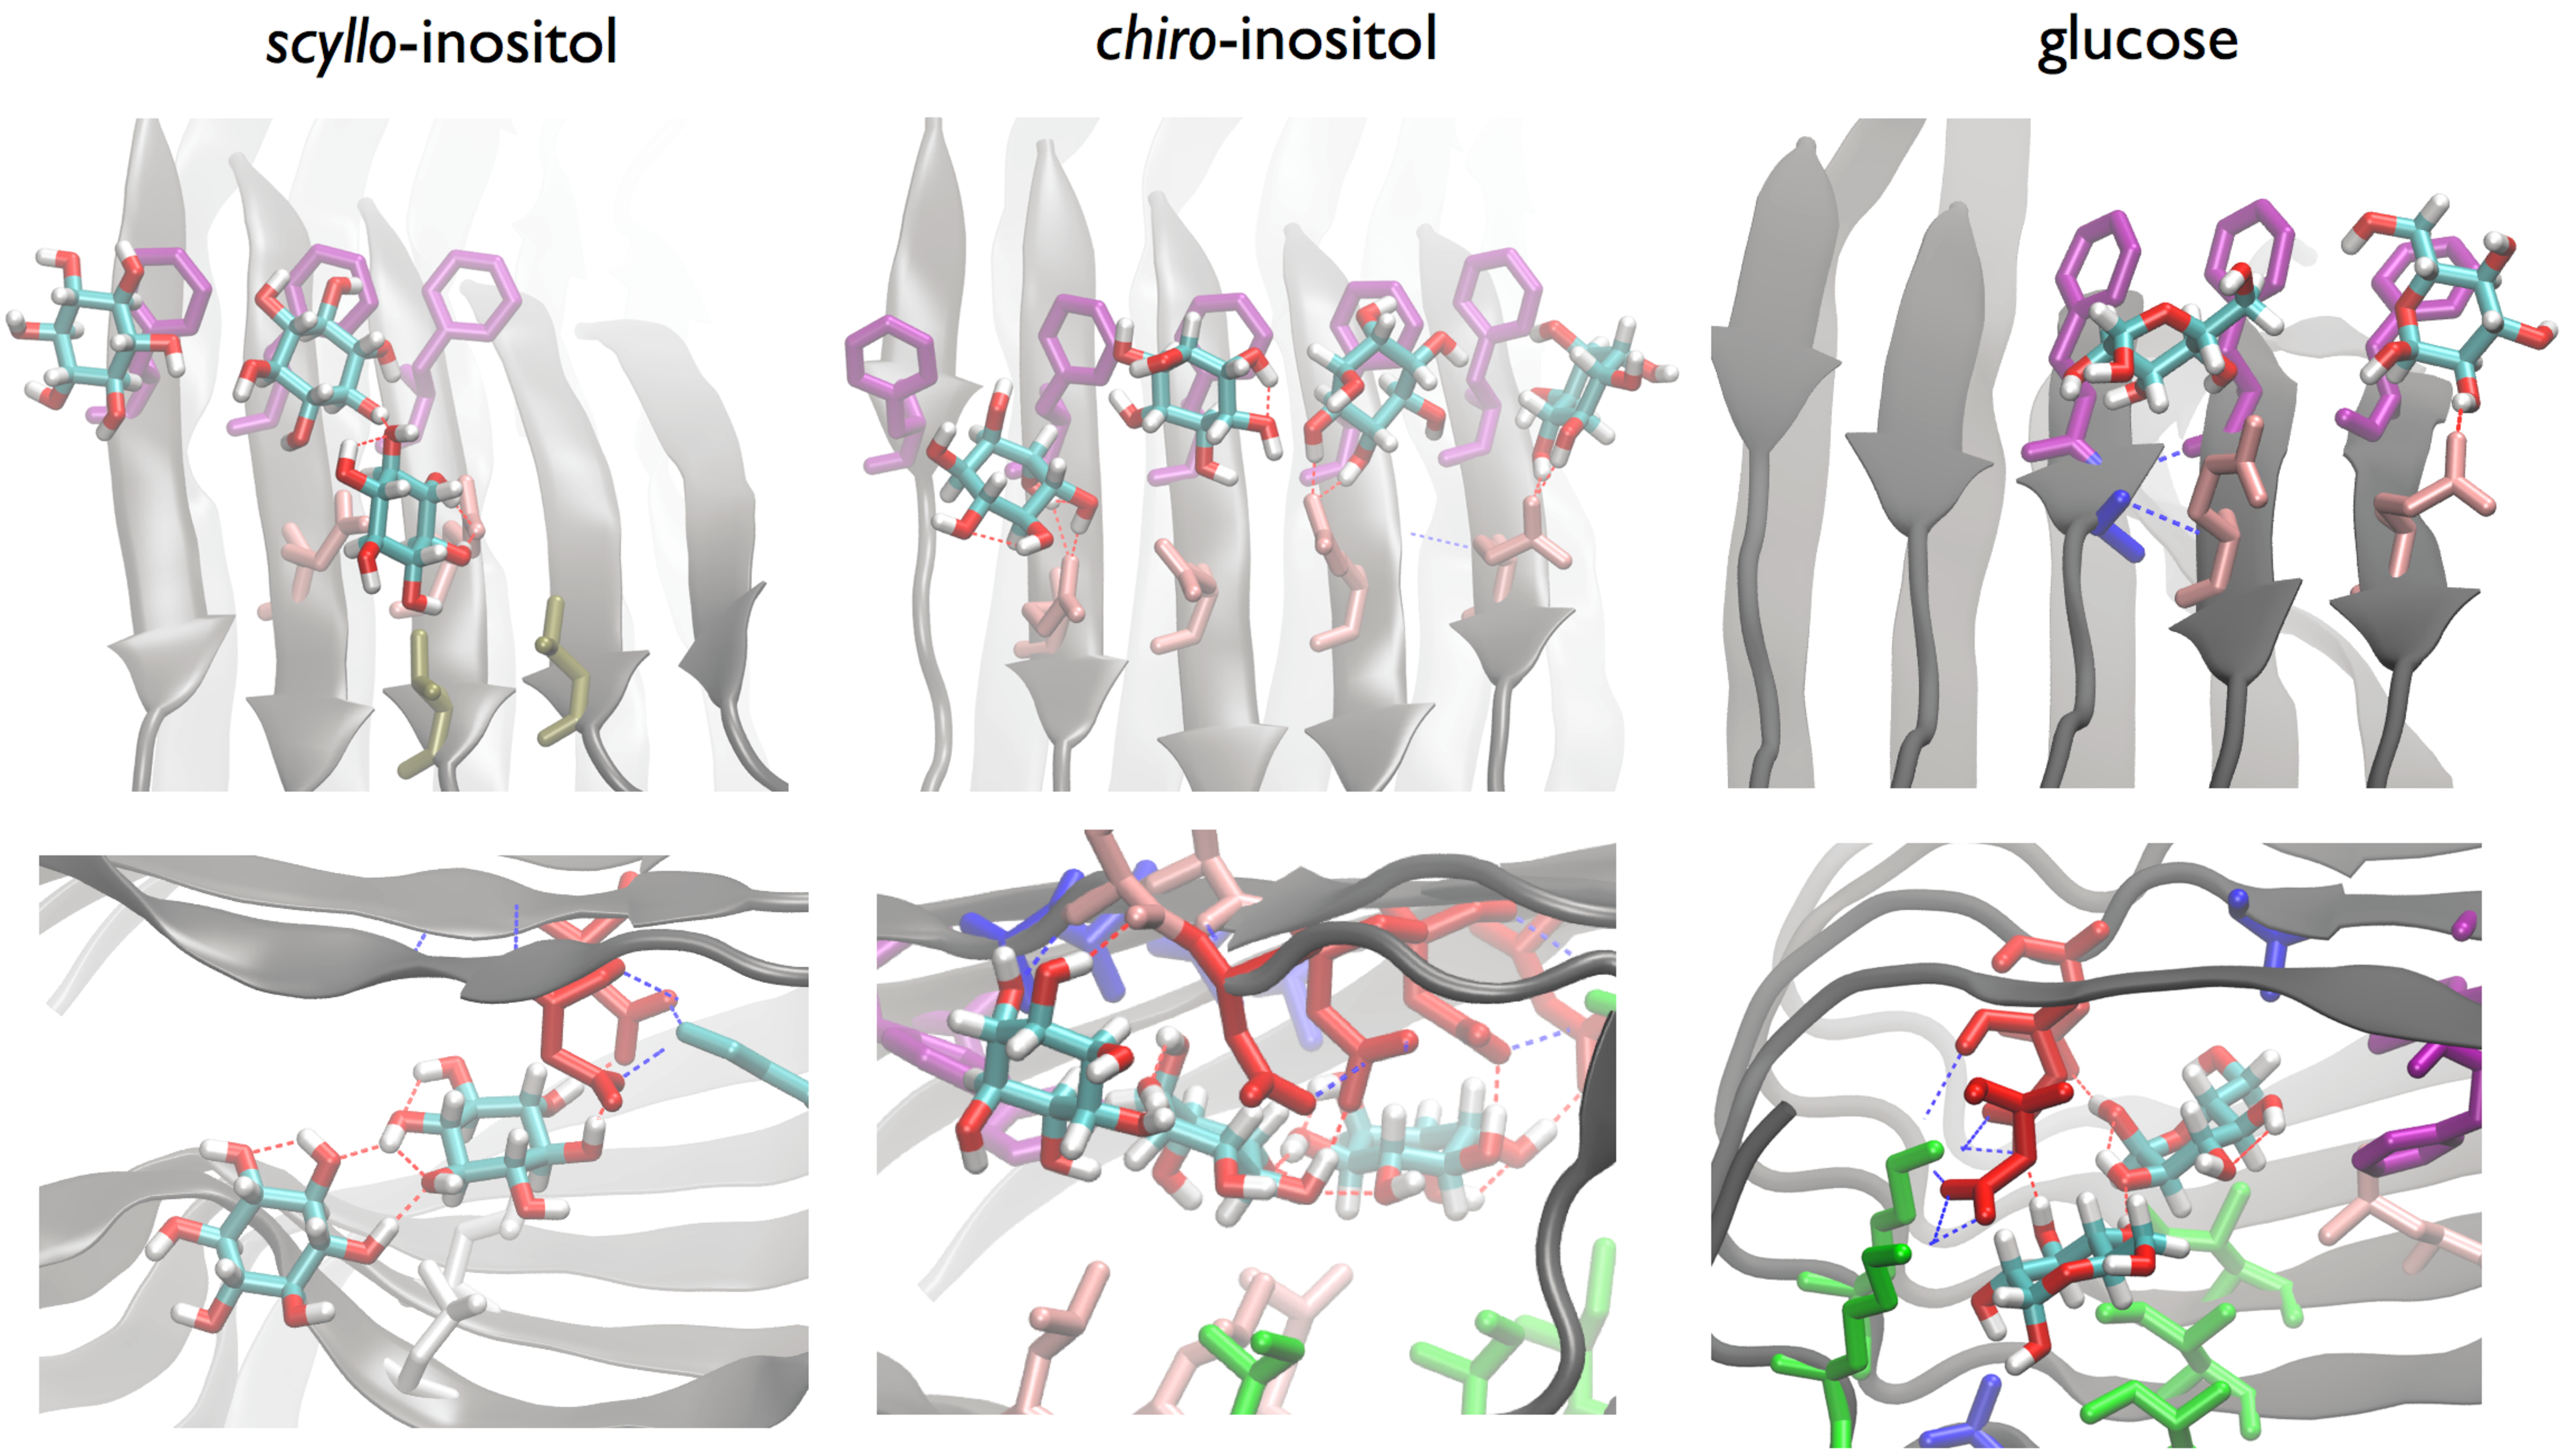
\includegraphics[width=6.5in]{figures/results3/detailed_binding_modes.pdf}
% \caption[Example binding modes of scyllo-inositol, chiro-inositol, and glucose to the protofibril]{Binding modes of scyllo-inositol, chiro-inositol and glucose to the $\beta$1 face (top row) and channel-like groove (bottom row). Residues that are within 4 \angstrom\ of a bound solute are represented in stick form. Protein is represented as a cartoon in gray.  Residues Phe, Glu, Asp, Lys and Ile are shown in colors purple, pink, red, green, and light green, respectively.}
% \label{fig:detailed_binding_modes}
%\end{figure}

%\begin{figure}[htbp]
%  \centering
%  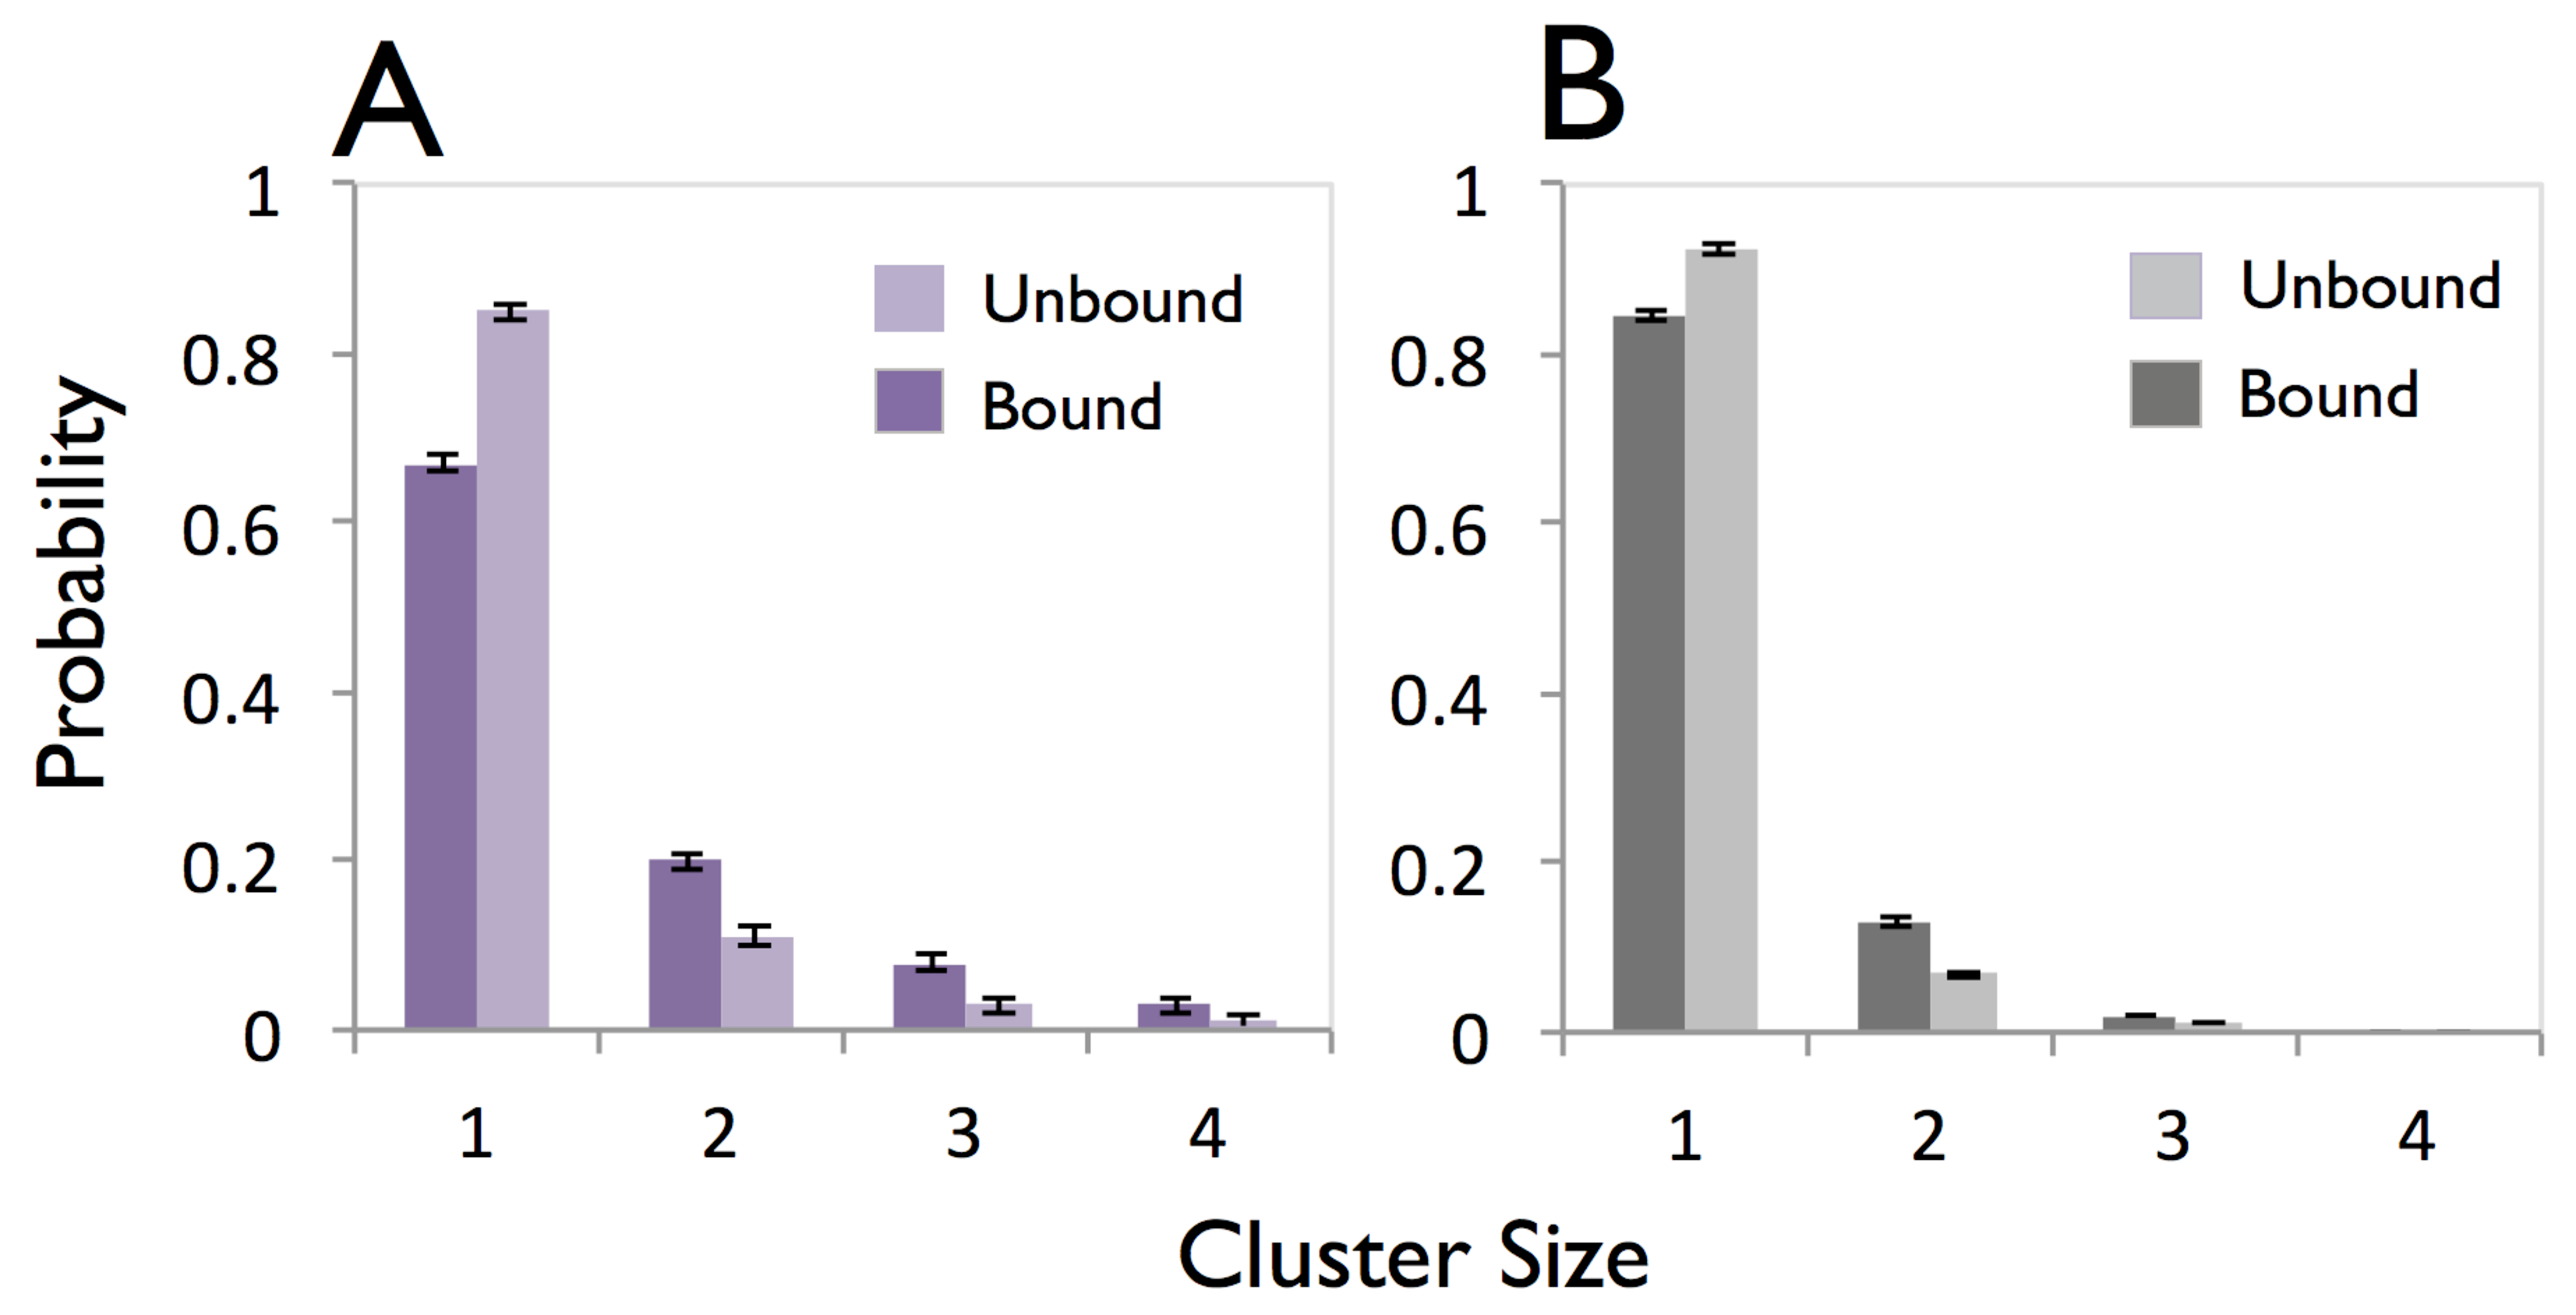
\includegraphics[width=6in]{figures/results3/clustered_binding.pdf}
%  \caption[Clustered binding of solutes at the surface of the protofibril]{Bound versus unbound cluster histograms for each solute.}
%  \label{fig:cluster_binding}
%\end{figure}

% Remove -- all of this information is already contained and is more clearly captured in the contact map
%\begin{figure}[htbp]
%  \centering
%  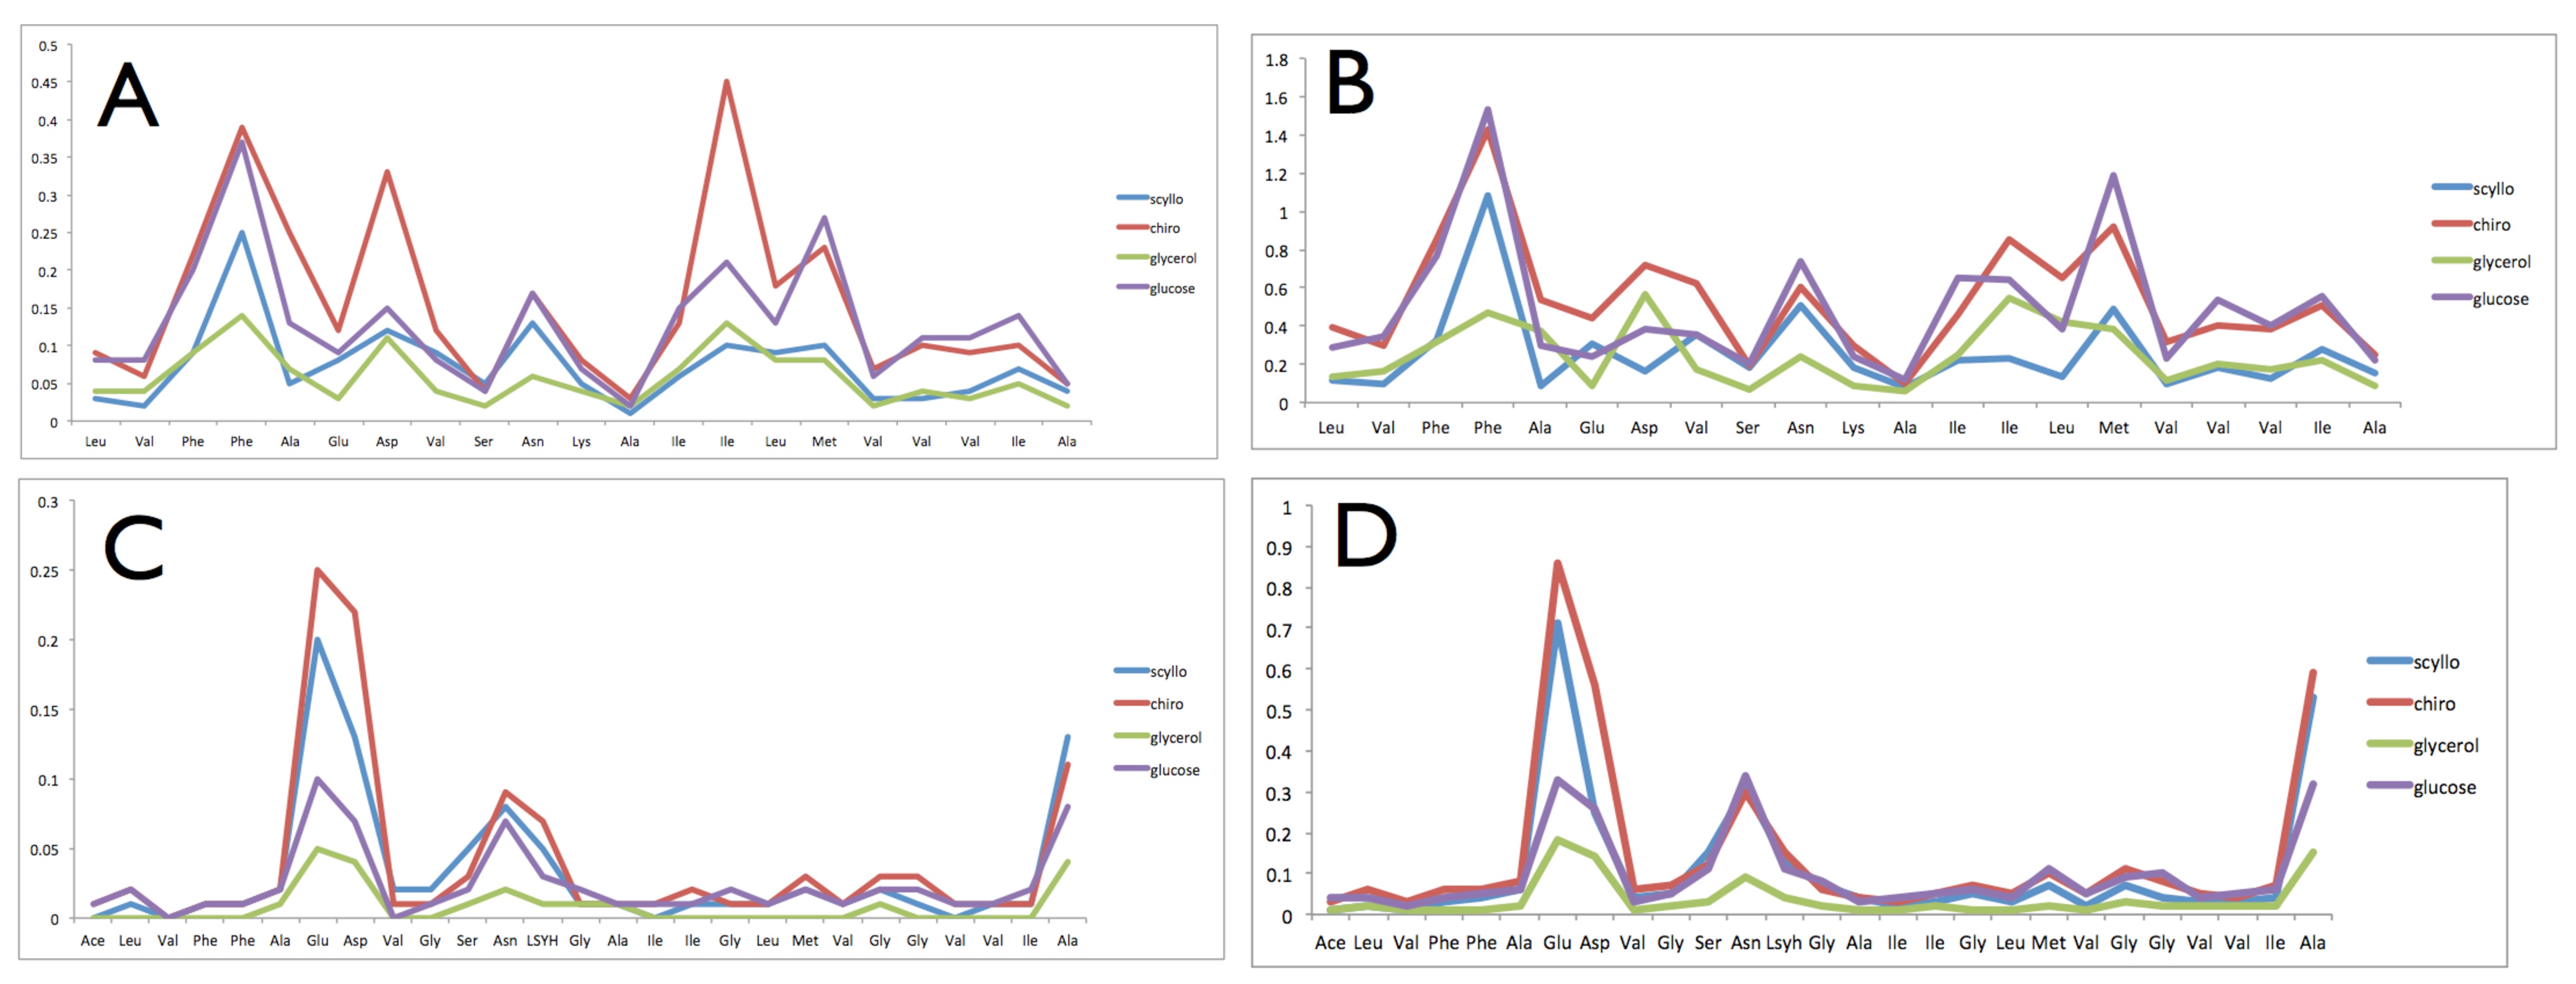
\includegraphics[width=6in]{figures/results3/binding_propensity_per_residue.pdf}
%  \caption[Binding propensity]{Binding propensity per residue of scyllo-inositol, chiro-inositol, glycerol and glucose. Nonpolar binding propensities are depicted in (A) and (B), and hydrogen bonding propensities in (C) and (D).}
%% Try to put nonpolar and hydrogen bonding for each ligand on separate panels. When put together it�s a little difficult to emphasize the differences
%  \label{fig:binding_propensity}
%\end{figure}



\begin{singlespace}
\addcontentsline{toc}{section}{Bibliography}
\bibliographystyle{elsart-num}
\bibliography{results3/results3}
\end{singlespace}

